%% This is file `tikz-sfc-doc.tex'
%% Version: 1.0.1
%% Version date: 2018-15-12
%% 
%% Copyright (C) 2018 by Luis Paulo Laus, laus@utfpr.edu.br
%%
%% This package can be redistributed and/or modified under the terms
%% of the LaTeX Project Public License distributed from CTAN
%% archives in directory macros/latex/base/lppl.txt; either
%% version 1 of the License, or (at your option) any later version,
%% with `The Package' referring to the software `tikzlibrarycircuits.plc.sfc.code.tex'
%% and its accompanying documentation and `The Copyright Holder' referring to
%% the person Luis Paulo Laus.
%% 
%% 
%% IMPORTANT NOTICE: 
%% 
%% For error reports, comments or suggestions in case of UNCHANGED 
%% versions send mail to:
%% laus@utfpr.edu.br
%% 
%%
\documentclass[a4paper]{ltxdoc}
\usepackage[hyphens]{url}
\usepackage[pdfborder={0 0 0}]{hyperref}
\usepackage[version=latest]{pgf}
\usepackage{calc,listings,tikz}
\usepackage{pdfpages}

\usepackage{hyperref}
\hypersetup{%
	colorlinks=false, % use true to enable colors below:
	linkcolor=blue,%red,
	filecolor=blue,%magenta,
	urlcolor=blue,%cyan,
	citecolor=blue,
	pdfborder=0 0 0,
}

% We need lots of libraries\ldots
\usetikzlibrary{backgrounds,circuits.logic.IEC}

\newif\ifgdccodebasic
\newif\ifgdccodeogdf

\usepackage[a4paper,left=2.25cm,right=2.25cm,top=2.5cm,bottom=2.5cm,nohead]{geometry}
\usepackage{amsmath,amssymb}
\usepackage{xxcolor}
\usepackage{pifont}
%%   \usepackage{tgpagella} % no ligatures (test)
\usepackage{makeidx}
\usepackage{enumitem}
\usepackage[T1]{fontenc}
\usepackage[latin9]{inputenc}


% Copyright 2006 by Till Tantau
%
% This file may be distributed and/or modified
%
% 1. under the LaTeX Project Public License and/or
% 2. under the GNU Free Documentation License.
%
% See the file doc/generic/pgf/licenses/LICENSE for more details.

% $Header: /cvsroot/pgf/pgf/doc/generic/pgf/macros/pgfmanual-en-macros.tex,v 1.81 2014/03/20 10:07:44 tantau Exp $


\providecommand\href[2]{\texttt{#1}}
\providecommand\hypertarget[2]{\texttt{#1}}
\providecommand\hyperlink[2]{\texttt{#1}}


\colorlet{examplefill}{yellow!80!black}
\definecolor{graphicbackground}{rgb}{0.96,0.96,0.8}
\definecolor{codebackground}{rgb}{0.9,0.9,1}

\newenvironment{pgfmanualentry}{\list{}{\leftmargin=2em\itemindent-\leftmargin\def\makelabel##1{\hss##1}}}{\endlist}
\newcommand\pgfmanualentryheadline[1]{\itemsep=0pt\parskip=0pt{\raggedright\item\strut{#1}\par}\topsep=0pt}
\newcommand\pgfmanualbody{\parskip3pt}

\let\origtexttt=\texttt
\def\texttt#1{{\def\textunderscore{\char`\_}\def\textbraceleft{\char`\{}\def\textbraceright{\char`\}}\origtexttt{#1}}}
\def\exclamationmarktext{!}
\def\atmarktext{@}

{
  \catcode`\|=12
  \gdef\pgfmanualnormalbar{|}
  \catcode`\|=13
  \AtBeginDocument{\gdef|{\ifmmode\pgfmanualnormalbar\else\expandafter\verb\expandafter|\fi}}
}



\newenvironment{pgflayout}[1]{
  \begin{pgfmanualentry}
    \pgfmanualentryheadline{%
      \pgfmanualpdflabel{#1}{}%
      \texttt{\string\pgfpagesuselayout\char`\{\declare{#1}\char`\}}\oarg{options}%
    }
    \index{#1@\protect\texttt{#1} layout}%
    \index{Page layouts!#1@\protect\texttt{#1}}%
    \pgfmanualbody
}
{
  \end{pgfmanualentry}
}


\newenvironment{command}[1]{
  \begin{pgfmanualentry}
    \extractcommand#1\@@
    \pgfmanualbody
}
{
  \end{pgfmanualentry}
}

\makeatletter

\def\includeluadocumentationof#1{
  \directlua{require 'pgf.manual.DocumentParser'}
  \directlua{pgf.manual.DocumentParser.include '#1'}
}

\newenvironment{luageneric}[4]{
  \pgfmanualentry
    \pgfmanualentryheadline{#4 \texttt{#1\declare{#2}}#3}
    \index{#2@\protect\texttt{#2} (Lua)}%
    \def\temp{#1}
    \ifx\temp\pgfutil@empty\else
      \index{#1@\protect\texttt{#1}!#2@\protect\texttt{#2} (Lua)}%
    \fi
  \pgfmanualbody
}{\endpgfmanualentry}

\newenvironment{luatable}[3]{
  \medskip
  \luageneric{#1}{#2}{ (declared in \texttt{#3})}{\textbf{Lua table}}
}{\endluageneric}

\newenvironment{luafield}[1]{
  \pgfmanualentry
    \pgfmanualentryheadline{Field \texttt{\declare{#1}}}
  \pgfmanualbody
}{\endpgfmanualentry}


\newenvironment{lualibrary}[1]{
  \pgfmanualentry
  \pgfmanualentryheadline{%
    \pgfmanualpdflabel{#1}{}%
    \textbf{Graph Drawing Library} \texttt{\declare{#1}}%
  }
    \index{#1@\protect\texttt{#1} graph drawing library}%
    \index{Libraries!#1@\protect\texttt{#1}}%
    \index{Graph drawing libraries!#1@\protect\texttt{#1}}%
    \vskip.25em
    {\ttfamily\char`\\usegdlibrary\char`\{\declare{#1}\char`\}\space\space \char`\%\space\space  \LaTeX\space and plain \TeX}\\
    {\ttfamily\char`\\usegdlibrary[\declare{#1}]\space \char`\%\space\space Con\TeX t}\smallskip\par
    \pgfmanualbody
}{\endpgfmanualentry}

\newenvironment{luadeclare}[4]{
  \pgfmanualentry
  \def\manual@temp@default{#3}%
  \def\manual@temp@initial{#4}%
  \def\manual@temp@{#3#4}%
  \pgfmanualentryheadline{%
    \pgfmanualpdflabel{#1}{}%
    {\ttfamily/graph
      drawing/\declare{#1}\opt{=}}\opt{#2}\hfill%
    \ifx\manual@temp@\pgfutil@empty\else%
    (\ifx\manual@temp@default\pgfutil@empty\else%
    default {\ttfamily #3}\ifx\manual@temp@initial\pgfutil@empty\else, \fi%
    \fi%
    \ifx\manual@temp@initial\pgfutil@empty\else%
    initially {\ttfamily #4}%
    \fi%
    )\fi%
  }%
  \index{#1@\protect\texttt{#1} key}%
  \pgfmanualbody
  \gdef\myname{#1}%
%  \keyalias{tikz}
%  \keyalias{tikz/graphs}
}{\endpgfmanualentry}

\newenvironment{luadeclarestyle}[4]{
  \pgfmanualentry
  \def\manual@temp@para{#2}%
  \def\manual@temp@default{#3}%
  \def\manual@temp@initial{#4}%
  \def\manual@temp@{#3#4}%
  \pgfmanualentryheadline{%
    \pgfmanualpdflabel{#1}{}%
    {\ttfamily/graph drawing/\declare{#1}}\ifx\manual@temp@para\pgfutil@empty\else\opt{\texttt=}\opt{#2}\fi\hfill%
    (style\ifx\manual@temp@\pgfutil@empty\else, %
    \ifx\manual@temp@default\pgfutil@empty\else%
    default {\ttfamily #3}\ifx\manual@temp@initial\pgfutil@empty\else, \fi%
    \fi%
    \ifx\manual@temp@initial\pgfutil@empty\else%
    initially {\ttfamily #4}%
    \fi%
    \fi)%
  }%
  \index{#1@\protect\texttt{#1} key}%
  \pgfmanualbody%
  \gdef\myname{#1}%
%  \keyalias{tikz}
%  \keyalias{tikz/graphs}
}{\endpgfmanualentry}

\newenvironment{luanamespace}[2]{
  \luageneric{#1}{#2}{}{\textbf{Lua namespace}}
}{\endluageneric}

\newenvironment{luafiledescription}[1]{}{}

\newenvironment{luacommand}[4]{
  \hypertarget{pgf/lua/#1}{\luageneric{#2}{#3}{\texttt{(#4)}}{\texttt{function}}}
}{\endluageneric}

\newenvironment{luaparameters}{\par\emph{Parameters:}%
  \parametercount=0\relax%
  \let\item=\parameteritem%
  \let\list=\restorelist%
}
{\par
}

\newenvironment{luareturns}{\par\emph{Returns:}%
  \parametercount=0\relax%
  \let\item=\parameteritem%
  \let\list=\restorelist%
}
{\par
}

\newcount\parametercount

\newenvironment{parameterdescription}{\unskip%
  \parametercount=0\relax%
  \let\item=\parameteritem%
  \let\list=\restorelist%
}
{\par
}
\let\saveditemcommand=\item
\let\savedlistcommand=\list
\def\denselist#1#2{\savedlistcommand{#1}{#2}\parskip0pt\itemsep0pt}
\def\restorelist{\let\item=\saveditemcommand\denselist}
\def\parameteritem{\pgfutil@ifnextchar[\parameteritem@{}}%}
\def\parameteritem@[#1]{\advance\parametercount by1\relax\hskip0.15em plus 1em\emph{\the\parametercount.}\kern1ex\def\test{#1}\ifx\test\pgfutil@empty\else#1\kern.5em\fi}

\makeatother
\newenvironment{commandlist}[1]{%
  \begin{pgfmanualentry}
  \foreach \xx in {#1} {%
    \expandafter\extractcommand\xx\@@
  }%
  \pgfmanualbody
}{%
  \end{pgfmanualentry}
}%
\makeatletter

% \begin{internallist}[register]{\pgf@xa}
% \end{internallist}
%
% \begin{internallist}[register]{\pgf@xa,\pgf@xb}
% \end{internallist}
\newenvironment{internallist}[2][register]{%
  \begin{pgfmanualentry}
  \foreach \xx in {#2} {%
    \expandafter\extractinternalcommand\expandafter{\xx}{#1}%
  }%
  \pgfmanualbody
}{%
  \end{pgfmanualentry}
}%
\def\extractinternalcommand#1#2{%
  \removeats{#1}%
  \pgfmanualentryheadline{%
    \pgfmanualpdflabel{\textbackslash\strippedat}{}%
    Internal #2 \declare{\texttt{\string#1}}}%
  \index{Internals!\strippedat @\protect\myprintocmmand{\strippedat}}%
  \index{\strippedat @\protect\myprintocmmand{\strippedat}}%
}

%% MW: START MATH MACROS
\def\mvar#1{{\ifmmode\textrm{\textit{#1}}\else\rmfamily\textit{#1}\fi}}

\makeatletter

\def\extractmathfunctionname#1{\extractmathfunctionname@#1(,)\tmpa\tmpb}
\def\extractmathfunctionname@#1(#2)#3\tmpb{\def\mathname{#1}}

\makeatother

\newenvironment{math-function}[1]{
  \def\mathdefaultname{#1}
  \extractmathfunctionname{#1}
  \edef\mathurl{{math:\mathname}}\expandafter\hypertarget\expandafter{\mathurl}{}%
  \begin{pgfmanualentry}
    \pgfmanualentryheadline{\texttt{#1}}%
    \index{\mathname @\protect\texttt{\mathname} math function}%
    \index{Math functions!\mathname @\protect\texttt{\mathname}}%
    \pgfmanualbody
}
{
  \end{pgfmanualentry}
}

\def\pgfmanualemptytext{}
\def\pgfmanualvbarvbar{\char`\|\char`\|}

\newenvironment{math-operator}[4][]{%
  \begin{pgfmanualentry}
  \csname math#3operator\endcsname{#2}{#4}
  \def\mathtest{#4}%
  \ifx\mathtest\pgfmanualemptytext%
    \def\mathtype{(#3 operator)}
  \else%
    \def\mathtype{(#3 operator; uses the \texttt{#4} function)}
  \fi%
  \pgfmanualentryheadline{\mathexample\hfill\mathtype}%
  \def\mathtest{#1}%
  \ifx\mathtest\pgfmanualemptytext%
    \index{#2@\protect\texttt{#2} #3 math operator}%
    \index{Math operators!#2@\protect\texttt{#2}}%
  \fi%
  \pgfmanualbody
}
{\end{pgfmanualentry}}

\newenvironment{math-operators}[5][]{%
  \begin{pgfmanualentry}
  \csname math#4operator\endcsname{#2}{#3}
  \def\mathtest{#5}%
  \ifx\mathtest\pgfmanualemptytext%
    \def\mathtype{(#4 operators)}
  \else%
    \def\mathtype{(#4 operators; use the \texttt{#5} function)}
  \fi%
  \pgfmanualentryheadline{\mathexample\hfill\mathtype}%
  \def\mathtest{#1}%
  \ifx\mathtest\pgfmanualemptytext%
    \index{#2#3@\protect\texttt{#2\protect\ #3} #4 math operators}%
    \index{Math operators!#2#3@\protect\texttt{#2\protect\ #3}}%
  \fi%
  \pgfmanualbody
}
{\end{pgfmanualentry}}

\def\mathinfixoperator#1#2{%
  \def\mathoperator{\texttt{#1}}%
  \def\mathexample{\mvar{x}\space\texttt{#1}\space\mvar{y}}%
}

\def\mathprefixoperator#1#2{%
  \def\mathoperator{\texttt{#1}}%
  \def\mathexample{\texttt{#1}\mvar{x}}%
}

\def\mathpostfixoperator#1#2{%
  \def\mathoperator{\texttt{#1}}
  \def\mathexample{\mvar{x}\texttt{#1}}%
}

\def\mathgroupoperator#1#2{%
  \def\mathoperator{\texttt{#1\ #2}}%
  \def\mathexample{\texttt{#1}\mvar{x}\texttt{#2}}%
}

\expandafter\let\csname matharray accessoperator\endcsname=\mathgroupoperator
\expandafter\let\csname matharrayoperator\endcsname=\mathgroupoperator

\def\mathconditionaloperator#1#2{%
  \def\mathoperator{#1\space#2}
  \def\mathexample{\mvar{x}\ \texttt{#1}\ \mvar{y}\ {\texttt{#2}}\ \mvar{z}}
}

\newcommand\mathcommand[1][\mathdefaultname]{%
  \expandafter\makemathcommand#1(\empty)\stop%
  \expandafter\extractcommand\mathcommandname\@@%
  \medskip
}
\makeatletter

\def\makemathcommand#1(#2)#3\stop{%
  \expandafter\def\expandafter\mathcommandname\expandafter{\csname pgfmath#1\endcsname}%
  \ifx#2\empty%
  \else%
    \@makemathcommand#2,\stop,
  \fi}
\def\@makemathcommand#1,{%
  \ifx#1\stop%
  \else%
    \expandafter\def\expandafter\mathcommandname\expandafter{\mathcommandname{\ttfamily\char`\{#1\char`\}}}%
    \expandafter\@makemathcommand%
  \fi}
\makeatother

\def\calcname{\textsc{calc}}

\newenvironment{math-keyword}[1]{
  \extracttikzmathkeyword#1@
  \begin{pgfmanualentry}
    \pgfmanualentryheadline{\texttt{\color{red}\mathname}\mathrest}%
    \index{\mathname @\protect\texttt{\mathname} tikz math function}%
    \index{TikZ math functions!\mathname @\protect\texttt{\mathname}}%
    \pgfmanualbody
}
{
  \end{pgfmanualentry}
}

\def\extracttikzmathkeyword#1#2@{%
  \def\mathname{#1}%
  \def\mathrest{#2}%
}

%% MW: END MATH MACROS


\def\extractcommand#1#2\@@{%
  \removeats{#1}%
  \pgfmanualentryheadline{%
    \pgfmanualpdflabel{\textbackslash\strippedat}{}%
    \declare{\texttt{\string#1}}#2%
  }%
  \index{\strippedat @\protect\myprintocmmand{\strippedat}}
}

\def\luaextractcommand#1#2\relax{%
  \declare{\texttt{\string#1}}#2\par%
%  \removeats{#1}%
 % \index{\strippedat @\protect\myprintocmmand{\strippedat}}
 % \pgfmanualpdflabel{\textbackslash\strippedat}{}%
}


% \begin{environment}{{name}\marg{arguments}}
\renewenvironment{environment}[1]{
  \begin{pgfmanualentry}
    \extractenvironement#1\@@
    \pgfmanualbody
}
{
  \end{pgfmanualentry}
}

\def\extractenvironement#1#2\@@{%
  \pgfmanualentryheadline{%
    \pgfmanualpdflabel{#1}{}%
    {\ttfamily\char`\\begin\char`\{\declare{#1}\char`\}}#2%
  }%
  \pgfmanualentryheadline{{\ttfamily\ \ }\meta{environment contents}}%
  \pgfmanualentryheadline{{\ttfamily\char`\\end\char`\{\declare{#1}\char`\}}}%
  \index{#1@\protect\texttt{#1} environment}%
  \index{Environments!#1@\protect\texttt{#1}}
}


\newenvironment{plainenvironment}[1]{
  \begin{pgfmanualentry}
    \extractplainenvironement#1\@@
    \pgfmanualbody
}
{
  \end{pgfmanualentry}
}

\def\extractplainenvironement#1#2\@@{%
  \pgfmanualentryheadline{{\ttfamily\declare{\char`\\#1}}#2}%
  \pgfmanualentryheadline{{\ttfamily\ \ }\meta{environment contents}}%
  \pgfmanualentryheadline{{\ttfamily\declare{\char`\\end#1}}}%
  \index{#1@\protect\texttt{#1} environment}%
  \index{Environments!#1@\protect\texttt{#1}}%
}


\newenvironment{contextenvironment}[1]{
  \begin{pgfmanualentry}
    \extractcontextenvironement#1\@@
    \pgfmanualbody
}
{
  \end{pgfmanualentry}
}

\def\extractcontextenvironement#1#2\@@{%
  \pgfmanualentryheadline{{\ttfamily\declare{\char`\\start#1}}#2}%
  \pgfmanualentryheadline{{\ttfamily\ \ }\meta{environment contents}}%
  \pgfmanualentryheadline{{\ttfamily\declare{\char`\\stop#1}}}%
  \index{#1@\protect\texttt{#1} environment}%
  \index{Environments!#1@\protect\texttt{#1}}}


\newenvironment{shape}[1]{
  \begin{pgfmanualentry}
    \pgfmanualentryheadline{%
      \pgfmanualpdflabel{#1}{}%
      \textbf{Shape} {\ttfamily\declare{#1}}%
    }%
    \index{#1@\protect\texttt{#1} shape}%
    \index{Shapes!#1@\protect\texttt{#1}}
    \pgfmanualbody
}
{
  \end{pgfmanualentry}
}

\newenvironment{pictype}[2]{
  \begin{pgfmanualentry}
    \pgfmanualentryheadline{%
      \pgfmanualpdflabel{#1}{}%
      \textbf{Pic type} {\ttfamily\declare{#1}#2}%
    }%
    \index{#1@\protect\texttt{#1} pic type}%
    \index{Pic Types!#1@\protect\texttt{#1}}
    \pgfmanualbody
}
{
  \end{pgfmanualentry}
}

\newenvironment{shading}[1]{
  \begin{pgfmanualentry}
    \pgfmanualentryheadline{%
      \pgfmanualpdflabel{#1}{}%
      \textbf{Shading} {\ttfamily\declare{#1}}}%
    \index{#1@\protect\texttt{#1} shading}%
    \index{Shadings!#1@\protect\texttt{#1}}
    \pgfmanualbody
}
{
  \end{pgfmanualentry}
}


\newenvironment{graph}[1]{
  \begin{pgfmanualentry}
    \pgfmanualentryheadline{%
      \pgfmanualpdflabel{#1}{}%
      \textbf{Graph} {\ttfamily\declare{#1}}}%
    \index{#1@\protect\texttt{#1} graph}%
    \index{Graphs!#1@\protect\texttt{#1}}
    \pgfmanualbody
}
{
  \end{pgfmanualentry}
}

\newenvironment{gdalgorithm}[2]{
  \begin{pgfmanualentry}
    \pgfmanualentryheadline{%
      \pgfmanualpdflabel{#1}{}%
      \textbf{Layout} {\ttfamily/graph drawing/\declare{#1}\opt{=}}\opt{\meta{options}}}%
    \index{#1@\protect\texttt{#1} layout}%
    \index{Layouts!#1@\protect\texttt{#1}}%
    \foreach \algo in {#2}
    {\edef\marshal{\noexpand\index{#2@\noexpand\protect\noexpand\texttt{#2} algorithm}}\marshal}%
    \index{Graph drawing layouts!#1@\protect\texttt{#1}}
    \item{\small alias {\ttfamily/tikz/#1}}\par
    \item{\small alias {\ttfamily/tikz/graphs/#1}}\par
    \item{\small Employs {\ttfamily algorithm=#2}}\par
    \pgfmanualbody
}
{
  \end{pgfmanualentry}
}

\newenvironment{dataformat}[1]{
  \begin{pgfmanualentry}
    \pgfmanualentryheadline{%
      \pgfmanualpdflabel{#1}{}%
      \textbf{Format} {\ttfamily\declare{#1}}}%
    \index{#1@\protect\texttt{#1} format}%
    \index{Formats!#1@\protect\texttt{#1}}
    \pgfmanualbody
}
{
  \end{pgfmanualentry}
}

\newenvironment{stylesheet}[1]{
  \begin{pgfmanualentry}
    \pgfmanualentryheadline{%
      \pgfmanualpdflabel{#1}{}%
      \textbf{Style sheet} {\ttfamily\declare{#1}}}%
    \index{#1@\protect\texttt{#1} style sheet}%
    \index{Style sheets!#1@\protect\texttt{#1}}
    \pgfmanualbody
}
{
  \end{pgfmanualentry}
}

\newenvironment{handler}[1]{
  \begin{pgfmanualentry}
    \extracthandler#1\@nil%
    \pgfmanualbody
}
{
  \end{pgfmanualentry}
}

\def\gobble#1{}
\def\extracthandler#1#2\@nil{%
  \pgfmanualentryheadline{%
    \pgfmanualpdflabel{/handlers/#1}{}%
    \textbf{Key handler} \meta{key}{\ttfamily/\declare{#1}}#2}%
  \index{\gobble#1@\protect\texttt{#1} handler}%
  \index{Key handlers!#1@\protect\texttt{#1}}
}


\makeatletter


\newenvironment{stylekey}[1]{
  \begin{pgfmanualentry}
    \def\extrakeytext{style, }
    \extractkey#1\@nil%
    \pgfmanualbody
}
{
  \end{pgfmanualentry}
}

\def\choicesep{$\vert$}%
\def\choicearg#1{\texttt{#1}}

\newif\iffirstchoice

% \mchoice{choice1,choice2,choice3}
\newcommand\mchoice[1]{%
  \begingroup
  \firstchoicetrue
  \foreach \mchoice@ in {#1} {%
    \iffirstchoice
      \global\firstchoicefalse
    \else
      \choicesep
    \fi
    \choicearg{\mchoice@}%
  }%
  \endgroup
}%

% \begin{key}{/path/x=value}
% \begin{key}{/path/x=value (initially XXX)}
% \begin{key}{/path/x=value (default XXX)}
\newenvironment{key}[1]{
  \begin{pgfmanualentry}
    \def\extrakeytext{}
    %\def\altpath{\emph{\color{gray}or}}%
    \extractkey#1\@nil%
    \pgfmanualbody
}
{
  \end{pgfmanualentry}
}

% \insertpathifneeded{a key}{/pgf} -> assign mykey={/pgf/a key}
% \insertpathifneeded{/tikz/a key}{/pgf} -> assign mykey={/tikz/a key}
%
% #1: the key
% #2: a default path (or empty)
\def\insertpathifneeded#1#2{%
  \def\insertpathifneeded@@{#2}%
  \ifx\insertpathifneeded@@\empty
    \def\mykey{#1}%
  \else
    \insertpathifneeded@#2\@nil
    \ifpgfutil@in@
      \def\mykey{#2/#1}%
    \else
      \def\mykey{#1}%
    \fi
  \fi
}%
\def\insertpathifneeded@#1#2\@nil{%
  \def\insertpathifneeded@@{#1}%
  \def\insertpathifneeded@@@{/}%
  \ifx\insertpathifneeded@@\insertpathifneeded@@@
    \pgfutil@in@true
  \else
    \pgfutil@in@false
  \fi
}%

% \begin{keylist}[default path]
%   {/path/option 1=value,/path/option 2=value2}
% \end{keylist}
\newenvironment{keylist}[2][]{%
  \begin{pgfmanualentry}
    \def\extrakeytext{}%
  \foreach \xx in {#2} {%
    \expandafter\insertpathifneeded\expandafter{\xx}{#1}%
    \expandafter\extractkey\mykey\@nil%
  }%
  \pgfmanualbody
}{%
  \end{pgfmanualentry}
}%

\def\extractkey#1\@nil{%
  \pgfutil@in@={#1}%
  \ifpgfutil@in@%
    \extractkeyequal#1\@nil
  \else%
    \pgfutil@in@{(initial}{#1}%
    \ifpgfutil@in@%
      \extractequalinitial#1\@nil%
    \else
      \pgfmanualentryheadline{%
      \def\mykey{#1}%
      \def\mypath{}%
      \gdef\myname{}%
      \firsttimetrue%
      \pgfmanualdecomposecount=0\relax%
      \decompose#1/\nil%
        {\ttfamily\declare{#1}}\hfill(\extrakeytext no value)}%
    \fi
  \fi%
}

\def\extractkeyequal#1=#2\@nil{%
  \pgfutil@in@{(default}{#2}%
  \ifpgfutil@in@%
    \extractdefault{#1}#2\@nil%
  \else%
    \pgfutil@in@{(initial}{#2}%
    \ifpgfutil@in@%
      \extractinitial{#1}#2\@nil%
    \else
      \pgfmanualentryheadline{%
        \def\mykey{#1}%
        \def\mypath{}%
        \gdef\myname{}%
        \firsttimetrue%
        \pgfmanualdecomposecount=0\relax%
        \decompose#1/\nil%
        {\ttfamily\declare{#1}=}#2\hfill(\extrakeytext no default)}%
    \fi%
  \fi%
}

\def\extractdefault#1#2(default #3)\@nil{%
  \pgfmanualentryheadline{%
    \def\mykey{#1}%
    \def\mypath{}%
    \gdef\myname{}%
    \firsttimetrue%
    \pgfmanualdecomposecount=0\relax%
    \decompose#1/\nil%
    {\ttfamily\declare{#1}\opt{=}}\opt{#2}\hfill (\extrakeytext default {\ttfamily#3})}%
}

\def\extractinitial#1#2(initially #3)\@nil{%
  \pgfmanualentryheadline{%
    \def\mykey{#1}%
    \def\mypath{}%
    \gdef\myname{}%
    \firsttimetrue%
    \pgfmanualdecomposecount=0\relax%
    \decompose#1/\nil%
    {\ttfamily\declare{#1}=}#2\hfill (\extrakeytext no default, initially {\ttfamily#3})}%
}

\def\extractequalinitial#1 (initially #2)\@nil{%
  \pgfmanualentryheadline{%
    \def\mykey{#1}%
    \def\mypath{}%
    \gdef\myname{}%
    \firsttimetrue%
    \pgfmanualdecomposecount=0\relax%
    \decompose#1/\nil%
    {\ttfamily\declare{#1}}\hfill (\extrakeytext initially {\ttfamily#2})}%
}

% Introduces a key alias '/#1/<name of current key>'
% to be used inside of \begin{key} ... \end{key}
\def\keyalias#1{\vspace{-3pt}\item{\small alias {\ttfamily/#1/\myname}}\vspace{-2pt}\par
  \pgfmanualpdflabel{/#1/\myname}{}%
}

\newif\iffirsttime
\newcount\pgfmanualdecomposecount

\makeatother

\def\decompose/#1/#2\nil{%
  \def\test{#2}%
  \ifx\test\empty%
    % aha.
    \index{#1@\protect\texttt{#1} key}%
    \index{\mypath#1@\protect\texttt{#1}}%
    \gdef\myname{#1}%
    \pgfmanualpdflabel{#1}{}
  \else%
    \advance\pgfmanualdecomposecount by1\relax%
    \ifnum\pgfmanualdecomposecount>2\relax%
      \decomposetoodeep#1/#2\nil%
    \else%
      \iffirsttime%
        \begingroup%
          % also make a pdf link anchor with full key path.
          \def\hyperlabelwithoutslash##1/\nil{%
            \pgfmanualpdflabel{##1}{}%
          }%
          \hyperlabelwithoutslash/#1/#2\nil%
        \endgroup%
        \def\mypath{#1@\protect\texttt{/#1/}!}%
        \firsttimefalse%
      \else%
        \expandafter\def\expandafter\mypath\expandafter{\mypath#1@\protect\texttt{#1/}!}%
      \fi%
      \def\firsttime{}%
      \decompose/#2\nil%
    \fi%
  \fi%
}

\def\decomposetoodeep#1/#2/\nil{%
  % avoid too-deep nesting in index
  \index{#1/#2@\protect\texttt{#1/#2} key}%
  \index{\mypath#1/#2@\protect\texttt{#1/#2}}%
  \decomposefindlast/#1/#2/\nil%
}
\makeatletter
\def\decomposefindlast/#1/#2\nil{%
  \def\test{#2}%
  \ifx\test\pgfutil@empty%
    \gdef\myname{#1}%
  \else%
    \decomposefindlast/#2\nil%
  \fi%
}
\makeatother
\def\indexkey#1{%
  \def\mypath{}%
  \decompose#1/\nil%
}

\newenvironment{predefinedmethod}[1]{
  \begin{pgfmanualentry}
    \extractpredefinedmethod#1\@nil
    \pgfmanualbody
}
{
  \end{pgfmanualentry}
}
\def\extractpredefinedmethod#1(#2)\@nil{%
  \pgfmanualentryheadline{%
    \pgfmanualpdflabel{#1}{}%
    Method \declare{\ttfamily #1}\texttt(#2\texttt) \hfill(predefined for all classes)}
  \index{#1@\protect\texttt{#1} method}%
  \index{Methods!#1@\protect\texttt{#1}}
}


\newenvironment{ooclass}[1]{
  \begin{pgfmanualentry}
    \def\currentclass{#1}
    \pgfmanualentryheadline{%
      \pgfmanualpdflabel{#1}{}%
      \textbf{Class} \declare{\texttt{#1}}}
    \index{#1@\protect\texttt{#1} class}%
    \index{Class #1@Class \protect\texttt{#1}}%
    \index{Classes!#1@\protect\texttt{#1}}
    \pgfmanualbody
}
{
  \end{pgfmanualentry}
}

\newenvironment{method}[1]{
  \begin{pgfmanualentry}
    \extractmethod#1\@nil
    \pgfmanualbody
}
{
  \end{pgfmanualentry}
}
\def\extractmethod#1(#2)\@nil{%
  \def\test{#1}
  \ifx\test\currentclass
    \pgfmanualentryheadline{%
      \pgfmanualpdflabel{#1}{}%
      Constructor \declare{\ttfamily #1}\texttt(#2\texttt)}
  \else
    \pgfmanualentryheadline{%
      \pgfmanualpdflabel{#1}{}%
      Method \declare{\ttfamily #1}\texttt(#2\texttt)}
  \fi
  \index{#1@\protect\texttt{#1} method}%
  \index{Methods!#1@\protect\texttt{#1}}
  \index{Class \currentclass!#1@\protect\texttt{#1}}%
}

\newenvironment{attribute}[1]{
  \begin{pgfmanualentry}
    \extractattribute#1\@nil
    \pgfmanualbody
}
{
  \end{pgfmanualentry}
}
\def\extractattribute#1=#2;\@nil{%
  \def\test{#2}%
  \ifx\test\@empty
    \pgfmanualentryheadline{%
      \pgfmanualpdflabel{#1}{}%
      Private attribute \declare{\ttfamily #1} \hfill (initially empty)}
  \else
    \pgfmanualentryheadline{%
      \pgfmanualpdflabel{#1}{}%
      Private attribute \declare{\ttfamily #1} \hfill (initially {\ttfamily #2})}
  \fi
  \index{#1@\protect\texttt{#1} attribute}%
  \index{Attributes!#1@\protect\texttt{#1}}
  \index{Class \currentclass!#1@\protect\texttt{#1}}%
}



\newenvironment{predefinednode}[1]{
  \begin{pgfmanualentry}
    \pgfmanualentryheadline{%
      \pgfmanualpdflabel{#1}{}%
      \textbf{Predefined node} {\ttfamily\declare{#1}}}%
    \index{#1@\protect\texttt{#1} node}%
    \index{Predefined node!#1@\protect\texttt{#1}}
    \pgfmanualbody
}
{
  \end{pgfmanualentry}
}

\newenvironment{coordinatesystem}[1]{
  \begin{pgfmanualentry}
    \pgfmanualentryheadline{%
      \pgfmanualpdflabel{#1}{}%
      \textbf{Coordinate system} {\ttfamily\declare{#1}}}%
    \index{#1@\protect\texttt{#1} coordinate system}%
    \index{Coordinate systems!#1@\protect\texttt{#1}}
    \pgfmanualbody
}
{
  \end{pgfmanualentry}
}

\newenvironment{snake}[1]{
  \begin{pgfmanualentry}
    \pgfmanualentryheadline{\textbf{Snake} {\ttfamily\declare{#1}}}%
    \index{#1@\protect\texttt{#1} snake}%
    \index{Snakes!#1@\protect\texttt{#1}}
    \pgfmanualbody
}
{
  \end{pgfmanualentry}
}

\newenvironment{decoration}[1]{
  \begin{pgfmanualentry}
    \pgfmanualentryheadline{\textbf{Decoration} {\ttfamily\declare{#1}}}%
    \index{#1@\protect\texttt{#1} decoration}%
    \index{Decorations!#1@\protect\texttt{#1}}
    \pgfmanualbody
}
{
  \end{pgfmanualentry}
}


\def\pgfmanualbar{\char`\|}
\makeatletter
\newenvironment{pathoperation}[3][]{
  \begin{pgfmanualentry}
    \def\pgfmanualtest{#1}%
    \pgfmanualentryheadline{%
      \ifx\pgfmanualtest\@empty%
        \pgfmanualpdflabel{#2}{}%
      \fi%
      \textcolor{gray}{{\ttfamily\char`\\path}\
        \ \dots}
      \declare{\texttt{\noligs{#2}}}#3\ \textcolor{gray}{\dots\texttt{;}}}%
    \ifx\pgfmanualtest\@empty%
      \index{#2@\protect\texttt{#2} path operation}%
      \index{Path operations!#2@\protect\texttt{#2}}%
    \fi%
    \pgfmanualbody
}
{
  \end{pgfmanualentry}
}
\newenvironment{datavisualizationoperation}[3][]{
  \begin{pgfmanualentry}
    \def\pgfmanualtest{#1}%
    \pgfmanualentryheadline{%
      \ifx\pgfmanualtest\@empty%
        \pgfmanualpdflabel{#2}{}%
      \fi%
      \textcolor{gray}{{\ttfamily\char`\\datavisualization}\
        \ \dots}
      \declare{\texttt{\noligs{#2}}}#3\ \textcolor{gray}{\dots\texttt{;}}}%
    \ifx\pgfmanualtest\@empty%
      \index{#2@\protect\texttt{#2} (data visualization)}%
      \index{Data visualization!#2@\protect\texttt{#2}}%
    \fi%
    \pgfmanualbody
}
{
  \end{pgfmanualentry}
}
\makeatother

\def\doublebs{\texttt{\char`\\\char`\\}}


\newenvironment{package}[1]{
  \begin{pgfmanualentry}
    \pgfmanualentryheadline{%
      \pgfmanualpdflabel{#1}{}%
      {\ttfamily\char`\\usepackage\char`\{\declare{#1}\char`\}\space\space \char`\%\space\space  \LaTeX}}
    \index{#1@\protect\texttt{#1} package}%
    \index{Packages and files!#1@\protect\texttt{#1}}%
    \pgfmanualentryheadline{{\ttfamily\char`\\input \declare{#1}.tex\space\space\space \char`\%\space\space  plain \TeX}}
    \pgfmanualentryheadline{{\ttfamily\char`\\usemodule[\declare{#1}]\space\space \char`\%\space\space  Con\TeX t}}
    \pgfmanualbody
}
{
  \end{pgfmanualentry}
}


\newenvironment{pgfmodule}[1]{
  \begin{pgfmanualentry}
    \pgfmanualentryheadline{%
      \pgfmanualpdflabel{#1}{}%
      {\ttfamily\char`\\usepgfmodule\char`\{\declare{#1}\char`\}\space\space\space
        \char`\%\space\space  \LaTeX\space and plain \TeX\space and pure pgf}}
    \index{#1@\protect\texttt{#1} module}%
    \index{Modules!#1@\protect\texttt{#1}}%
    \pgfmanualentryheadline{{\ttfamily\char`\\usepgfmodule[\declare{#1}]\space\space \char`\%\space\space  Con\TeX t\space and pure pgf}}
    \pgfmanualbody
}
{
  \end{pgfmanualentry}
}

\newenvironment{pgflibrary}[1]{
  \begin{pgfmanualentry}
    \pgfmanualentryheadline{%
      \pgfmanualpdflabel{#1}{}%
      \textbf{\tikzname\ Library} \texttt{\declare{#1}}}
    \index{#1@\protect\texttt{#1} library}%
    \index{Libraries!#1@\protect\texttt{#1}}%
    \vskip.25em%
    {{\ttfamily\char`\\usepgflibrary\char`\{\declare{#1}\char`\}\space\space\space
        \char`\%\space\space  \LaTeX\space and plain \TeX\space and pure pgf}}\\
    {{\ttfamily\char`\\usepgflibrary[\declare{#1}]\space\space \char`\%\space\space  Con\TeX t\space and pure pgf}}\\
    {{\ttfamily\char`\\usetikzlibrary\char`\{\declare{#1}\char`\}\space\space
        \char`\%\space\space  \LaTeX\space and plain \TeX\space when using \tikzname}}\\
    {{\ttfamily\char`\\usetikzlibrary[\declare{#1}]\space
        \char`\%\space\space  Con\TeX t\space when using \tikzname}}\\[.5em]
    \pgfmanualbody
}
{
  \end{pgfmanualentry}
}

\newenvironment{purepgflibrary}[1]{
  \begin{pgfmanualentry}
    \pgfmanualentryheadline{%
      \pgfmanualpdflabel{#1}{}%
      \textbf{{\small PGF} Library} \texttt{\declare{#1}}}
    \index{#1@\protect\texttt{#1} library}%
    \index{Libraries!#1@\protect\texttt{#1}}%
    \vskip.25em%
    {{\ttfamily\char`\\usepgflibrary\char`\{\declare{#1}\char`\}\space\space\space
        \char`\%\space\space  \LaTeX\space and plain \TeX}}\\
    {{\ttfamily\char`\\usepgflibrary[\declare{#1}]\space\space \char`\%\space\space  Con\TeX t}}\\[.5em]
    \pgfmanualbody
}
{
  \end{pgfmanualentry}
}

\newenvironment{tikzlibrary}[1]{
  \begin{pgfmanualentry}
    \pgfmanualentryheadline{%
      \pgfmanualpdflabel{#1}{}%
      \textbf{\tikzname\ Library} \texttt{\declare{#1}}}
    \index{#1@\protect\texttt{#1} library}%
    \index{Libraries!#1@\protect\texttt{#1}}%
    \vskip.25em%
    {{\ttfamily\char`\\usetikzlibrary\char`\{\declare{#1}\char`\}\space\space \char`\%\space\space  \LaTeX\space and plain \TeX}}\\
    {{\ttfamily\char`\\usetikzlibrary[\declare{#1}]\space \char`\%\space\space Con\TeX t}}\\[.5em]
    \pgfmanualbody
}
{
  \end{pgfmanualentry}
}



\newenvironment{filedescription}[1]{
  \begin{pgfmanualentry}
    \pgfmanualentryheadline{File {\ttfamily\declare{#1}}}%
    \index{#1@\protect\texttt{#1} file}%
    \index{Packages and files!#1@\protect\texttt{#1}}%
    \pgfmanualbody
}
{
  \end{pgfmanualentry}
}


\newenvironment{packageoption}[1]{
  \begin{pgfmanualentry}
    \pgfmanualentryheadline{{\ttfamily\char`\\usepackage[\declare{#1}]\char`\{pgf\char`\}}}
    \index{#1@\protect\texttt{#1} package option}%
    \index{Package options for \textsc{pgf}!#1@\protect\texttt{#1}}%
    \pgfmanualbody
}
{
  \end{pgfmanualentry}
}



\newcommand\opt[1]{{\color{black!50!green}#1}}
\newcommand\ooarg[1]{{\ttfamily[}\meta{#1}{\ttfamily]}}

\def\opt{\afterassignment\pgfmanualopt\let\next=}
\def\pgfmanualopt{\ifx\next\bgroup\bgroup\color{black!50!green}\else{\color{black!50!green}\next}\fi}



\def\beamer{\textsc{beamer}}
\def\pdf{\textsc{pdf}}
\def\eps{\texttt{eps}}
\def\pgfname{\textsc{pgf}}
\def\tikzname{Ti\emph{k}Z}
\def\pstricks{\textsc{pstricks}}
\def\prosper{\textsc{prosper}}
\def\seminar{\textsc{seminar}}
\def\texpower{\textsc{texpower}}
\def\foils{\textsc{foils}}

{
  \makeatletter
  \global\let\myempty=\@empty
  \global\let\mygobble=\@gobble
  \catcode`\@=12
  \gdef\getridofats#1@#2\relax{%
    \def\getridtest{#2}%
    \ifx\getridtest\myempty%
      \expandafter\def\expandafter\strippedat\expandafter{\strippedat#1}
    \else%
      \expandafter\def\expandafter\strippedat\expandafter{\strippedat#1\protect\printanat}
      \getridofats#2\relax%
    \fi%
  }

  \gdef\removeats#1{%
    \let\strippedat\myempty%
    \edef\strippedtext{\stripcommand#1}%
    \expandafter\getridofats\strippedtext @\relax%
  }

  \gdef\stripcommand#1{\expandafter\mygobble\string#1}
}

\def\printanat{\char`\@}

\def\declare{\afterassignment\pgfmanualdeclare\let\next=}
\def\pgfmanualdeclare{\ifx\next\bgroup\bgroup\color{red!75!black}\else{\color{red!75!black}\next}\fi}


\let\textoken=\command
\let\endtextoken=\endcommand

\def\myprintocmmand#1{\texttt{\char`\\#1}}

\def\example{\par\smallskip\noindent\textit{Example: }}
\def\themeauthor{\par\smallskip\noindent\textit{Theme author: }}


\def\indexoption#1{%
  \index{#1@\protect\texttt{#1} option}%
  \index{Graphic options and styles!#1@\protect\texttt{#1}}%
}

\def\itemcalendaroption#1{\item \declare{\texttt{#1}}%
  \index{#1@\protect\texttt{#1} date test}%
  \index{Date tests!#1@\protect\texttt{#1}}%
}



\def\class#1{\list{}{\leftmargin=2em\itemindent-\leftmargin\def\makelabel##1{\hss##1}}%
\extractclass#1@\par\topsep=0pt}
\def\endclass{\endlist}
\def\extractclass#1#2@{%
\item{{{\ttfamily\char`\\documentclass}#2{\ttfamily\char`\{\declare{#1}\char`\}}}}%
  \index{#1@\protect\texttt{#1} class}%
  \index{Classes!#1@\protect\texttt{#1}}}

\def\partname{Part}

\makeatletter
\def\index@prologue{\section*{Index}\addcontentsline{toc}{section}{Index}
  This index only contains automatically generated entries. A good
  index should also contain carefully selected keywords. This index is
  not a good index.
  \bigskip
}
\c@IndexColumns=2
  \def\theindex{\@restonecoltrue
    \columnseprule \z@  \columnsep 29\p@
    \twocolumn[\index@prologue]%
       \parindent -30pt
       \columnsep 15pt
       \parskip 0pt plus 1pt
       \leftskip 30pt
       \rightskip 0pt plus 2cm
       \small
       \def\@idxitem{\par}%
    \let\item\@idxitem \ignorespaces}
  \def\endtheindex{\onecolumn}
\def\noindexing{\let\index=\@gobble}


\newenvironment{arrowtipsimple}[1]{
  \begin{pgfmanualentry}
    \pgfmanualentryheadline{\textbf{Arrow Tip Kind} {\ttfamily#1}}
    \index{#1@\protect\texttt{#1} arrow tip}%
    \index{Arrow tips!#1@\protect\texttt{#1}}%
    \def\currentarrowtype{#1}
    \pgfmanualbody}
{
  \end{pgfmanualentry}
}

\newenvironment{arrowtip}[4]{
  \begin{pgfmanualentry}
    \pgfmanualentryheadline{\textbf{Arrow Tip Kind} {\ttfamily#1}}
    \index{#1@\protect\texttt{#1} arrow tip}%
    \index{Arrow tips!#1@\protect\texttt{#1}}%
    \pgfmanualbody
    \def\currentarrowtype{#1}
    \begin{minipage}[t]{10.25cm}
      #2
    \end{minipage}\hskip5mm\begin{minipage}[t]{4.75cm}
      \leavevmode\vskip-2em
    \tikz{
      \draw [black!50,line width=5mm,-{#1[#3,color=black]}] (-4,0) -- (0,0);
      \foreach \action in {#4}
      { \expandafter\processaction\action\relax }
    }
    \end{minipage}\par\smallskip
  }
{
  \end{pgfmanualentry}
}

\newenvironment{arrowcap}[5]{
  \begin{pgfmanualentry}
    \pgfmanualentryheadline{\textbf{Arrow Tip Kind} {\ttfamily#1}}
    \index{#1@\protect\texttt{#1} arrow tip}%
    \index{Arrow tips!#1@\protect\texttt{#1}}%
    \pgfmanualbody
    \def\currentarrowtype{#1}
    \begin{minipage}[t]{10.25cm}
      #2
    \end{minipage}\hskip5mm\begin{minipage}[t]{4.75cm}
      \leavevmode\vskip-2em
    \tikz{
      \path [tips, line width=10mm,-{#1[#3,color=black]}] (-4,0) -- (0,0);
      \draw [line width=10mm,black!50] (-3,0) -- (#5,0);
      \foreach \action in {#4}
      { \expandafter\processaction\action\relax }
    }
    \end{minipage}\par\smallskip
  }
{
  \end{pgfmanualentry}
}

\def\processaction#1=#2\relax{
  \expandafter\let\expandafter\pgf@temp\csname manual@action@#1\endcsname
  \ifx\pgf@temp\relax\else
    \pgf@temp#2/0/\relax
  \fi
}
\def\manual@action@length#1/#2/#3\relax{%
  \draw [red,|<->|,semithick,xshift=#2] ([yshift=4pt]current bounding
  box.north -| -#1,0) coordinate (last length) -- node
  [above=-2pt] {|length|} ++(#1,0);
}
\def\manual@action@width#1/#2/#3\relax{%
  \draw [overlay, red,|<->|,semithick] (.5,-#1/2) -- node [below,sloped] {|width|} (.5,#1/2);
}
\def\manual@action@inset#1/#2/#3\relax{%
  \draw [red,|<->|,semithick,xshift=#2] ([yshift=-4pt]current bounding
  box.south -| last length) -- node [below] {|inset|} ++(#1,0);
}

\newenvironment{arrowexamples}
{\begin{tabbing}
    \hbox to \dimexpr\linewidth-5.5cm\relax{\emph{Appearance of the below at line width} \hfil} \=
     \hbox to 1.9cm{\emph{0.4pt}\hfil} \= \hbox to 2cm{\emph{0.8pt}\hfil} \= \emph{1.6pt} \\
  }
{\end{tabbing}\vskip-1em}

\newenvironment{arrowcapexamples}
{\begin{tabbing}
    \hbox to \dimexpr\linewidth-5.5cm\relax{\emph{Appearance of the below at line width} \hfil} \=
     \hbox to 1.9cm{\emph{1ex}\hfil} \= \hbox to 2cm{\emph{1em}\hfil} \\
  }
{\end{tabbing}\vskip-1em}

\def\arrowcapexample#1[#2]{\def\temp{#1}\ifx\temp\pgfutil@empty\arrowcapexample@\currentarrowtype[{#2}]\else\arrowcapexample@#1[{#2}]\fi}
\def\arrowcapexample@#1[#2]{%
  {\sfcode`\.1000\small\texttt{#1[#2]}} \>
  \kern-.5ex\tikz [baseline,>={#1[#2]}] \draw [line
  width=1ex,->] (0,.5ex) -- (2em,.5ex);  \>
  \kern-.5em\tikz [baseline,>={#1[#2]}] \draw [line
  width=1em,->] (0,.5ex) -- (2em,.5ex);  \\
}

\def\arrowexample#1[#2]{\def\temp{#1}\ifx\temp\pgfutil@empty\arrowexample@\currentarrowtype[{#2}]\else\arrowexample@#1[{#2}]\fi}
\def\arrowexample@#1[#2]{%
  {\sfcode`\.1000\small\texttt{#1[#2]}} \>
  \tikz [baseline,>={#1[#2]}] \draw [line
  width=0.4pt,->] (0,.5ex) -- (2em,.5ex); thin \>
  \tikz [baseline,>={#1[#2]}] \draw [line
  width=0.8pt,->] (0,.5ex) -- (2em,.5ex); \textbf{thick} \>
  \tikz [baseline,>={#1[#2]}] \draw [line
  width=1.6pt,->] (0,.5ex) -- (3em,.5ex); \\
}
\def\arrowexampledup[#1]{\arrowexample[{#1] \currentarrowtype[}]}
\def\arrowexampledupdot[#1]{\arrowexample[{#1] . \currentarrowtype[}]}

\def\arrowexampledouble#1[#2]{\def\temp{#1}\ifx\temp\pgfutil@empty\arrowexampledouble@\currentarrowtype[{#2}]\else\arrowexampledouble@#1[{#2}]\fi}
\def\arrowexampledouble@#1[#2]{%
  {\sfcode`\.1000\small\texttt{#1[#2]} on double line} \>
  \tikz [baseline,>={#1[#2]}]
    \draw [double equal sign distance,line width=0.4pt,->] (0,.5ex) -- (2em,.5ex); thin \>
  \tikz [baseline,>={#1[#2]}]
    \draw [double equal sign distance,line width=0.8pt,->] (0,.5ex) -- (2em,.5ex); \textbf{thick} \>
  \tikz [baseline,>={#1[#2]}]
    \draw [double equal sign distance, line width=1.6pt,->] (0,.5ex) -- (3em,.5ex); \\
}



\newcommand\symarrow[1]{%
  \index{#1@\protect\texttt{#1} arrow tip}%
  \index{Arrow tips!#1@\protect\texttt{#1}}%
  \texttt{#1}& yields thick
  \begin{tikzpicture}[arrows={#1-#1},thick,baseline]
    \useasboundingbox (-1mm,-0.5ex) rectangle (1.1cm,2ex);
    \fill [black!15] (1cm,-.5ex) rectangle (1.1cm,1.5ex) (-1mm,-.5ex) rectangle (0mm,1.5ex) ;
    \draw (0pt,.5ex) -- (1cm,.5ex);
  \end{tikzpicture} and thin
  \begin{tikzpicture}[arrows={#1-#1},thin,baseline]
    \useasboundingbox (-1mm,-0.5ex) rectangle (1.1cm,2ex);
    \fill [black!15] (1cm,-.5ex) rectangle (1.1cm,1.5ex) (-1mm,-.5ex) rectangle (0mm,1.5ex) ;
    \draw (0pt,.5ex) -- (1cm,.5ex);
  \end{tikzpicture}
}
\newcommand\symarrowdouble[1]{%
  \index{#1@\protect\texttt{#1} arrow tip}%
  \index{Arrow tips!#1@\protect\texttt{#1}}%
  \texttt{#1}& yields thick
  \begin{tikzpicture}[arrows={#1-#1},thick,baseline]
    \useasboundingbox (-1mm,-0.5ex) rectangle (1.1cm,2ex);
    \fill [black!15] (1cm,-.5ex) rectangle (1.1cm,1.5ex) (-1mm,-.5ex) rectangle (0mm,1.5ex) ;
    \draw (0pt,.5ex) -- (1cm,.5ex);
  \end{tikzpicture}
  and thin
  \begin{tikzpicture}[arrows={#1-#1},thin,baseline]
    \useasboundingbox (-1mm,-0.5ex) rectangle (1.1cm,2ex);
    \fill [black!15] (1cm,-.5ex) rectangle (1.1cm,1.5ex) (-1mm,-.5ex) rectangle (0mm,1.5ex) ;
    \draw (0pt,.5ex) -- (1cm,.5ex);
  \end{tikzpicture}, double
  \begin{tikzpicture}[arrows={#1-#1},thick,baseline]
    \useasboundingbox (-1mm,-0.5ex) rectangle (1.1cm,2ex);
    \fill [black!15] (1cm,-.5ex) rectangle (1.1cm,1.5ex) (-1mm,-.5ex) rectangle (0mm,1.5ex) ;
    \draw[double,double equal sign distance] (0pt,.5ex) -- (1cm,.5ex);
  \end{tikzpicture} and
  \begin{tikzpicture}[arrows={#1-#1},thin,baseline]
    \useasboundingbox (-1mm,-0.5ex) rectangle (1.1cm,2ex);
    \fill [black!15] (1cm,-.5ex) rectangle (1.1cm,1.5ex) (-1mm,-.5ex) rectangle (0mm,1.5ex) ;
    \draw[double,double equal sign distance] (0pt,.5ex) -- (1cm,.5ex);
  \end{tikzpicture}
}

\newcommand\sarrow[2]{%
  \index{#1@\protect\texttt{#1} arrow tip}%
  \index{Arrow tips!#1@\protect\texttt{#1}}%
  \index{#2@\protect\texttt{#2} arrow tip}%
  \index{Arrow tips!#2@\protect\texttt{#2}}%
  \texttt{#1-#2}& yields thick
  \begin{tikzpicture}[arrows={#1-#2},thick,baseline]
    \useasboundingbox (-1mm,-0.5ex) rectangle (1.1cm,2ex);
    \fill [black!15] (1cm,-.5ex) rectangle (1.1cm,1.5ex) (-1mm,-.5ex) rectangle (0mm,1.5ex) ;
    \draw (0pt,.5ex) -- (1cm,.5ex);
  \end{tikzpicture} and thin
  \begin{tikzpicture}[arrows={#1-#2},thin,baseline]
    \useasboundingbox (-1mm,-0.5ex) rectangle (1.1cm,2ex);
    \fill [black!15] (1cm,-.5ex) rectangle (1.1cm,1.5ex) (-1mm,-.5ex) rectangle (0mm,1.5ex) ;
    \draw (0pt,.5ex) -- (1cm,.5ex);
  \end{tikzpicture}
}

\newcommand\sarrowdouble[2]{%
  \index{#1@\protect\texttt{#1} arrow tip}%
  \index{Arrow tips!#1@\protect\texttt{#1}}%
  \index{#2@\protect\texttt{#2} arrow tip}%
  \index{Arrow tips!#2@\protect\texttt{#2}}%
  \texttt{#1-#2}& yields thick
  \begin{tikzpicture}[arrows={#1-#2},thick,baseline]
    \useasboundingbox (-1mm,-0.5ex) rectangle (1.1cm,2ex);
    \fill [black!15] (1cm,-.5ex) rectangle (1.1cm,1.5ex) (-1mm,-.5ex) rectangle (0mm,1.5ex) ;
    \draw (0pt,.5ex) -- (1cm,.5ex);
  \end{tikzpicture} and thin
  \begin{tikzpicture}[arrows={#1-#2},thin,baseline]
    \useasboundingbox (-1mm,-0.5ex) rectangle (1.1cm,2ex);
    \fill [black!15] (1cm,-.5ex) rectangle (1.1cm,1.5ex) (-1mm,-.5ex) rectangle (0mm,1.5ex) ;
    \draw (0pt,.5ex) -- (1cm,.5ex);
  \end{tikzpicture}, double
  \begin{tikzpicture}[arrows={#1-#2},thick,baseline]
    \useasboundingbox (-1mm,-0.5ex) rectangle (1.1cm,2ex);
    \fill [black!15] (1cm,-.5ex) rectangle (1.1cm,1.5ex) (-1mm,-.5ex) rectangle (0mm,1.5ex) ;
    \draw[double,double equal sign distance] (0pt,.5ex) -- (1cm,.5ex);
  \end{tikzpicture} and
  \begin{tikzpicture}[arrows={#1-#2},thin,baseline]
    \useasboundingbox (-1mm,-0.5ex) rectangle (1.1cm,2ex);
    \fill [black!15] (1cm,-.5ex) rectangle (1.1cm,1.5ex) (-1mm,-.5ex) rectangle (0mm,1.5ex) ;
    \draw[double,double equal sign distance] (0pt,.5ex) -- (1cm,.5ex);
  \end{tikzpicture}
}

\newcommand\carrow[1]{%
  \index{#1@\protect\texttt{#1} arrow tip}%
  \index{Arrow tips!#1@\protect\texttt{#1}}%
  \texttt{#1}& yields for line width 1ex
  \begin{tikzpicture}[arrows={#1-#1},line width=1ex,baseline]
    \useasboundingbox (-1mm,-0.5ex) rectangle (1.6cm,2ex);
    \fill [black!15] (1.5cm,-.5ex) rectangle (1.6cm,1.5ex) (-1mm,-.5ex) rectangle (0mm,1.5ex) ;
    \draw (0pt,.5ex) -- (1.5cm,.5ex);
  \end{tikzpicture}
}
\def\myvbar{\char`\|}
\newcommand\plotmarkentry[1]{%
  \index{#1@\protect\texttt{#1} plot mark}%
  \index{Plot marks!#1@\protect\texttt{#1}}
  \texttt{\char`\\pgfuseplotmark\char`\{\declare{\noligs{#1}}\char`\}} &
  \tikz\draw[color=black!25] plot[mark=#1,mark options={fill=examplefill,draw=black}] coordinates{(0,0) (.5,0.2) (1,0) (1.5,0.2)};\\
}
\newcommand\plotmarkentrytikz[1]{%
  \index{#1@\protect\texttt{#1} plot mark}%
  \index{Plot marks!#1@\protect\texttt{#1}}
  \texttt{mark=\declare{\noligs{#1}}} & \tikz\draw[color=black!25]
  plot[mark=#1,mark options={fill=examplefill,draw=black}]
    coordinates {(0,0) (.5,0.2) (1,0) (1.5,0.2)};\\
}



\ifx\scantokens\@undefined
  \PackageError{pgfmanual-macros}{You need to use extended latex
    (elatex) or (pdfelatex) to process this document}{}
\fi

\begingroup
\catcode`|=0
\catcode`[= 1
\catcode`]=2
\catcode`\{=12
\catcode `\}=12
\catcode`\\=12 |gdef|find@example#1\end{codeexample}[|endofcodeexample[#1]]
|endgroup

% define \returntospace.
%
% It should define NEWLINE as {}, spaces and tabs as \space.
\begingroup
\catcode`\^=7
\catcode`\^^M=13
\catcode`\^^I=13
\catcode`\ =13%
\gdef\returntospace{\catcode`\ =13\def {\space}\catcode`\^^I=13\def^^I{\space}}
\gdef\showreturn{\show^^M}
\endgroup

\begingroup
\catcode`\%=13
\catcode`\^^M=13
\gdef\commenthandler{\catcode`\%=13\def%{\@gobble@till@return}}
\gdef\@gobble@till@return#1^^M{}
\gdef\@gobble@till@return@ignore#1^^M{\ignorespaces}
\gdef\typesetcomment{\catcode`\%=13\def%{\@typeset@till@return}}
\gdef\@typeset@till@return#1^^M{{\def%{\char`\%}\textsl{\char`\%#1}}\par}
\endgroup

% Define tab-implementation functions
%   \codeexample@tabinit@replacementchars@
% and
%   \codeexample@tabinit@catcode@
%
% They should ONLY be used in case that tab replacement is active.
%
% This here is merely a preparation step.
%
% Idea:
% \codeexample@tabinit@catcode@ will make TAB active
% and
% \codeexample@tabinit@replacementchars@ will insert as many spaces as
% /codeexample/tabsize contains.
{
\catcode`\^^I=13
% ATTENTION: do NOT use tabs in these definitions!!
\gdef\codeexample@tabinit@replacementchars@{%
 \begingroup
 \count0=\pgfkeysvalueof{/codeexample/tabsize}\relax
 \toks0={}%
 \loop
 \ifnum\count0>0
  \advance\count0 by-1
  \toks0=\expandafter{\the\toks0\ }%
 \repeat
 \xdef\codeexample@tabinit@replacementchars@@{\the\toks0}%
 \endgroup
 \let^^I=\codeexample@tabinit@replacementchars@@
}%
\gdef\codeexample@tabinit@catcode@{\catcode`\^^I=13}%
}%

% Called after any options have been set. It assigns
%   \codeexample@tabinit@catcode
% and
%   \codeexample@tabinit@replacementchars
% which are used inside of
%\begin{codeexample}
% ...
%\end{codeexample}
%
% \codeexample@tabinit@catcode  is either \relax or it makes tab
% active.
%
% \codeexample@tabinit@replacementchars is either \relax or it inserts
% a proper replacement sequence for tabs (as many spaces as
% configured)
\def\codeexample@tabinit{%
  \ifnum\pgfkeysvalueof{/codeexample/tabsize}=0\relax
    \let\codeexample@tabinit@replacementchars=\relax
    \let\codeexample@tabinit@catcode=\relax
  \else
    \let\codeexample@tabinit@catcode=\codeexample@tabinit@catcode@
    \let\codeexample@tabinit@replacementchars=\codeexample@tabinit@replacementchars@
  \fi
}

\newif\ifpgfmanualtikzsyntaxhilighting

\pgfqkeys{/codeexample}{%
  width/.code=  {\setlength\codeexamplewidth{#1}},
  graphic/.code=  {\colorlet{graphicbackground}{#1}},
  code/.code=  {\colorlet{codebackground}{#1}},
  execute code/.is if=code@execute,
  code only/.code=  {\code@executefalse},
  pre/.store in=\code@pre,
  post/.store in=\code@post,
  % #1 is the *complete* environment contents as it shall be
  % typeset. In particular, the catcodes are NOT the normal ones.
  typeset listing/.code=  {#1},
  render instead/.store in=\code@render,
  vbox/.code=  {\def\code@pre{\vbox\bgroup\setlength{\hsize}{\linewidth-6pt}}\def\code@post{\egroup}},
  ignorespaces/.code=  {\let\@gobble@till@return=\@gobble@till@return@ignore},
  leave comments/.code=  {\def\code@catcode@hook{\catcode`\%=12}\let\commenthandler=\relax\let\typesetcomment=\relax},
  tabsize/.initial=0,% FIXME : this here is merely used for indentation. It is just a TAB REPLACEMENT.
  every codeexample/.style={width=4cm+7pt, tikz syntax=true},
  from file/.code={\codeexamplefromfiletrue\def\codeexamplesource{#1}},
  tikz syntax/.is if=pgfmanualtikzsyntaxhilighting,
}


\newread\examplesource


% Opening, reading and closing the results file

\def\opensource#1{
  \immediate\openin\examplesource=#1
}
\def\do@codeexamplefromfile{%
  \immediate\openin\examplesource\expandafter{\codeexamplesource}%
  \def\examplelines{}%
  \readexamplelines
  \closein\examplesource
  \expandafter\endofcodeexample\expandafter{\examplelines}%
}

\def\readexamplelines{
  \ifeof\examplesource%
  \else
    \immediate\read\examplesource to \exampleline
    \expandafter\expandafter\expandafter\def\expandafter\expandafter\expandafter\examplelines\expandafter\expandafter\expandafter{\expandafter\examplelines\exampleline}
    \expandafter\readexamplelines%
  \fi
}

\let\code@pre\pgfutil@empty
\let\code@post\pgfutil@empty
\let\code@render\pgfutil@empty
\def\code@catcode@hook{}

\newif\ifcodeexamplefromfile
\newdimen\codeexamplewidth
\newif\ifcode@execute
\newbox\codeexamplebox
\def\codeexample[#1]{%
  \begingroup%
  \code@executetrue
  \pgfqkeys{/codeexample}{every codeexample,#1}%
  \pgfmanualswitchoncolors%
  \ifcodeexamplefromfile\begingroup\fi
  \codeexample@tabinit% assigns \codeexample@tabinit@[catcode,replacementchars]
  \parindent0pt
  \begingroup%
  \par%
  \medskip%
  \let\do\@makeother%
  \dospecials%
  \obeylines%
  \@vobeyspaces%
  \catcode`\%=13%
  \catcode`\^^M=13%
  \code@catcode@hook%
  \codeexample@tabinit@catcode
  \relax%
  \ifcodeexamplefromfile%
    \expandafter\do@codeexamplefromfile%
  \else%
    \expandafter\find@example%
  \fi}
\def\endofcodeexample#1{%
  \endgroup%
  \ifcode@execute%
    \setbox\codeexamplebox=\hbox{%
      \ifx\code@render\pgfutil@empty%
      {%
        {%
          \returntospace%
          \commenthandler%
          \xdef\code@temp{#1}% removes returns and comments
        }%
        \catcode`\^^M=9%
        \colorbox{graphicbackground}{\color{black}\ignorespaces%
          \code@pre\expandafter\scantokens\expandafter{\code@temp\ignorespaces}\code@post\ignorespaces}%
      }%
      \else%
        \colorbox{graphicbackground}{\color{black}\ignorespaces%
          \code@render}%
      \fi%
    }%
    \ifdim\wd\codeexamplebox>\codeexamplewidth%
      \def\code@start{\par}%
      \def\code@flushstart{}\def\code@flushend{}%
      \def\code@mid{\parskip2pt\par\noindent}%
      \def\code@width{\linewidth-6pt}%
      \def\code@end{}%
    \else%
      \def\code@start{%
        \linewidth=\textwidth%
        \parshape \@ne 0pt \linewidth
        \leavevmode%
        \hbox\bgroup}%
      \def\code@flushstart{\hfill}%
      \def\code@flushend{\hbox{}}%
      \def\code@mid{\hskip6pt}%
      \def\code@width{\linewidth-12pt-\codeexamplewidth}%
      \def\code@end{\egroup}%
    \fi%
    \code@start%
    \noindent%
    \begin{minipage}[t]{\codeexamplewidth}\raggedright
      \hrule width0pt%
      \footnotesize\vskip-1em%
      \code@flushstart\box\codeexamplebox\code@flushend%
      \vskip-1ex
      \leavevmode%
    \end{minipage}%
  \else%
    \def\code@mid{\par}
    \def\code@width{\linewidth-6pt}
    \def\code@end{}
  \fi%
  \code@mid%
  \colorbox{codebackground}{%
    \pgfkeysvalueof{/codeexample/prettyprint/base color}%
    \begin{minipage}[t]{\code@width}%
      {%
        \let\do\@makeother
        \dospecials
        \frenchspacing\@vobeyspaces
        \normalfont\ttfamily\footnotesize
        \typesetcomment%
        \codeexample@tabinit@replacementchars
        \@tempswafalse
        \def\par{%
          \if@tempswa
          \leavevmode \null \@@par\penalty\interlinepenalty
          \else
          \@tempswatrue
          \ifhmode\@@par\penalty\interlinepenalty\fi
          \fi}%
        \obeylines
        \everypar \expandafter{\the\everypar \unpenalty}%
        \pgfkeysvalueof{/codeexample/typeset listing/.@cmd}{#1}\pgfeov
      }
    \end{minipage}}%
  \code@end%
  \par%
  \medskip
  \endcodeexample\endgroup
}

\def\endcodeexample{\endgroup}


\makeatother

\usepackage{pgfmanual}


% autoxref is now always on

% \makeatletter
% % \pgfautoxrefs will be defined by 'make dist'
% \pgfutil@ifundefined{pgfautoxrefs}{%
%   \renewcommand\pgfmanualpdflabel[3][]{#3}% NO-OP
%   \def\pgfmanualpdfref#1#2{#2}%
%   \pgfkeys{
%     /pdflinks/codeexample links=false,% DISABLED.
%   }%
% }{}
% \makeatother

\newdimen\pgfmanualcslinkpreskip

% Styling of the pretty printer
\pgfkeys{
  /codeexample/syntax hilighting/.style={
    /codeexample/prettyprint/key name/.code={\textcolor{keycolor}{\pgfmanualpdfref{##1}{\noligs{##1}}}},
    /codeexample/prettyprint/key name with handler/.code 2 args={\textcolor{keycolor}{\pgfmanualpdfref{##1}{\noligs{##1}}}/\textcolor{blue!70!black}{\pgfmanualpdfref{/handlers/##2}{\noligs{##2}}}},
    /codeexample/prettyprint/key value display only/.code={\textcolor{keycolor}{{\itshape{\let\pgfmanualwordstartup\relax\pgfmanualprettyprintcode{##1}}}}},
    /codeexample/prettyprint/cs/.code={\textcolor{cscolor}{\pgfmanualcslinkpreskip4.25pt\pgfmanualpdfref{##1}{\noligs{##1}}}},
    /codeexample/prettyprint/cs with args/.code 2 args={\textcolor{black}{\pgfmanualcslinkpreskip4.25pt\pgfmanualpdfref{##1}{\noligs{##1}}}\{\textcolor{black}{\pgfmanualprettyprintcode{##2}}\pgfmanualclosebrace},
    /codeexample/prettyprint/cs arguments/pgfkeys/.initial=1,
    /codeexample/prettyprint/cs/pgfkeys/.code 2 args={\textcolor{black}{\pgfmanualcslinkpreskip4.25pt\pgfmanualpdfref{##1}{\noligs{##1}}}\{\textcolor{black}{\pgfmanualprettyprintpgfkeys{##2}}\pgfmanualclosebrace},
    /codeexample/prettyprint/cs arguments/begin/.initial=1,
    /codeexample/prettyprint/cs/begin/.code 2 args={\textcolor{black}{##1}\{\textcolor{cscolor}{\pgfmanualpdfref{##2}{\noligs{##2}}}\pgfmanualclosebrace},
    /codeexample/prettyprint/cs arguments/end/.initial=1,
    /codeexample/prettyprint/cs/end/.code 2 args={\textcolor{black}{##1}\{\textcolor{cscolor}{\pgfmanualpdfref{##2}{\noligs{##2}}}\pgfmanualclosebrace},
    /codeexample/prettyprint/word/.code={\pgfmanualwordstartup{\begingroup\pgfkeyssetvalue{/pdflinks/search key prefixes in}{}\pgfmanualpdfref{##1}{\noligs{##1}}\endgroup}},
    /codeexample/prettyprint/point/.code={\textcolor{pointcolor}{\noligs{##1}}},%
    /codeexample/prettyprint/point with cs/.code 2 args={\textcolor{pointcolor}{(\pgfmanualpdfref{##1}{\noligs{##1}}:\noligs{##2}}},%
    /codeexample/prettyprint/comment font=\itshape,
    /codeexample/prettyprint/base color/.initial=\color{basecolor},
    /pdflinks/render hyperlink/.code={%
      {\setbox0=\hbox{##1}%
        \rlap{{\color{linkcolor}\dimen0\wd0\advance\dimen0by-\pgfmanualcslinkpreskip\hskip\pgfmanualcslinkpreskip\vrule width\dimen0 height-1pt depth1.6pt}}%
        \box0%
      }%
    }
  },/codeexample/syntax hilighting
}

\colorlet{keycolor}{black}
\colorlet{cscolor}{black}
\colorlet{pointcolor}{black}
\colorlet{basecolor}{black}
\colorlet{linkcolor}{black!8}

\def\pgfmanualswitchoncolors{%
  \colorlet{keycolor}{green!50!black}%
  \colorlet{cscolor}{blue!70!black}
  \colorlet{pointcolor}{violet}
  \colorlet{basecolor}{black!55}
  \colorlet{linkcolor}{white}
}

\makeatletter

\def\pgfmanualwordstartup{\textcolor{black}}

\def\noligs#1{\pgfmanualnoligs#1\kern0pt--\pgf@stop}%
\def\pgfmanualnoligs#1--{%
  \pgfutil@ifnextchar\pgf@stop{#1\pgfutil@gobble}{#1-\kern0pt-\kern0pt\pgfmanualnoligs}%
}
\makeatother


%%% Local Variables:
%%% mode: latex
%%% TeX-master: "beameruserguide"
%%% End:
    % Borrowed from TikZ/PGF

\makeindex

\makeatletter
\renewcommand*\l@section[2]{%
  \ifnum \c@tocdepth >\z@
    \addpenalty\@secpenalty
    \addvspace{1.0em \@plus\p@}%
    \setlength\@tempdima{2.5em}%
    \begingroup
      \parindent \z@ \rightskip \@pnumwidth
      \parfillskip -\@pnumwidth
      \leavevmode \bfseries
      \advance\leftskip\@tempdima
      \hskip -\leftskip
      #1\nobreak\hfil \nobreak\hb@xt@\@pnumwidth{\hss #2}\par
    \endgroup
  \fi}
\renewcommand*\l@subsection{\@dottedtocline{2}{2.5em}{3.3em}}
\renewcommand*\l@subsubsection{\@dottedtocline{3}{5.8em}{4.2em}}
\def\@pnumwidth{2.2em}
\makeatother


% Global styles:
\tikzset{
  every plot/.style={prefix=plots/pgf-},
  shape example/.style={
    color=black!30,
    draw,
    fill=yellow!30,
    line width=.5cm,
    inner xsep=2.5cm,
    inner ysep=0.5cm}
}

%%%%%%%%%%%%%%%%%%%%%%%%%%%%%%%%%%%%%%%%%%%%%%%%%%%%%%%%%%%%%%%%%%%%%
%
% This file really starts here, all the above is for pgfmanual 
% compatibility
% \usetikzlibrary{circuits.plc.sfc}
\input ../tex/tikzlibrarycircuits.plc.sfc.code
% \usetikzlibrary{circuits.plc.ladder} % used in examples
\input ../../tikz-ladder/tex/tikzlibrarycircuits.plc.ladder.code
\sloppy

\begin{document}

\title{Typesetting Sequential Function Chart (SFC) with \LaTeX{} and \tikzname{}}
\author{Luis Paulo Laus\\e-mail: \texttt{laus@utfpr.edu.br}}
\date{Version: 1.0, Version date: 2018-01-16}

\maketitle

\section{Abstract}
Sequential Function Chart (SFC) describes the behaviour of a control program. It is derived from Petri Nets and GRAFCET. This package contains a set of symbols that simplifies the drawing of SFC diagrams with emphasis in readability and in agreement with the international standard IEC~61\,131-3. It extends the \tikzname-library |circuits| which defines general keys for creating circuits. All graphic elements of SFC are supported by |tikz-sfc|: steps (normal and initial), transitions, actions and actions qualifiers (with and without time duration) are supported. The placement of all actions associated with a step is done automatically. Comments can also be placed automatically in a suitable location near the element they refer to. The final appearance of each element can be fine-tuned individually or in group.

\section{Introduction\label{sec:introduction}}
IEC~61\,131-3 Sequential Function Chart (SFC) describes the behaviour of a control program. It is derived from Petri Nets and IEC~60\,848 GRAFCET, with the changes necessary to convert the representation from a documentation standard to a set of execution control elements.

The GRAFCET language, described by IEC~60\,848, has served as foundation of SFC
language of IEC standard 61\,131-3, but the syntax and the semantics defined by each of the two standards are nevertheless distinct because their scopes are different. GRAFCET is regarded as a \emph{specification language} and SFC as an \emph{implementation of the language for programming}. Many features of GRAFCET are not supported in SFC, but all GRAFCET functionalities can be implemented in SFC, although not directly. Particularly, assignation condition, time dependent assignation condition, delayed action, time limited action, stored actions, action on activation, action on deactivation, action at the clearing and action on event are all done, one way or another, in SFC using action qualifiers\footnote{This package typesets qualifiers in the agreement with the international standard IEC 61 131-3/2013.  The lack of qualifier support in GRAFCET and in particular in the |grafcet| package is the main reason to have a different package for SFC.} (mainly). Consequently, the graphical representation of those features is fairly different. If you are interested in GRAFCET, refer to Robert Papanicola's |grafcet| package\footnote{The |grafcet| package uses a very different approach in the user interface. It is based in writing down a sequence of macro calls. The |tikz-sfc| uses the \tikzname-library |circuits| interface in which you place symbols along a path.}.

SFC structures the internal organization of a program, and helps to decompose a control problem into manageable parts, while maintaining the overview.

SFC consists of steps and transitions interconnected by directed links. Associated with each step is a set of actions, and with each transition is associated a transition condition. Each step represents a particular state of the systems being controlled. A transition is associated with a condition, which, when true, causes the step before the transition to be deactivated, and the next step to be activated. Steps are linked to actions, performing a certain control action. An action qualifier can be used in the association of a step with an action. Each element can be programmed in any of the standard languages defined in IEC~61\,131-3, including SFC itself.

Steps (normal and initial), transitions, actions and actions qualifiers (with and without time) are shown in the example below for a star-delta motor starter with dead time.

\begin{codeexample}[width=4.5cm]
\begin{tikzpicture}[circuit plc sfc,thick,x=2.6\tikzcircuitssizeunit,
  y=1.3\tikzcircuitssizeunit,sfcaqw=8\tikzcircuitssizeunit]
  \draw (0,0)
     to [flow direction={pos=0.95}] ++(0,-1)
     to [sfcstepi={info=O}] ++(0,-4)
     node [sfctransition={info=b1 AND NOT b0}] {}
     to [sfcstep={info=I, 
            sfcaction={info=K1,qualifier=N},
            sfcaction={info=K2,qualifier=L,time=T\#3s},
            sfcaction={info=K3,qualifier=D,time=T\#3s400ms}}] ++(0,-4)
     node [sfctransition={info=b0}]{}
     |- ++(-1,-1) |- (0,0);
\end{tikzpicture}
\end{codeexample}

\section{SFC Library}
\begin{pgflibrary}{circuits.plc.sfc}
This library provides graphics for Sequential Function Chart (SFC) related to programable controllers (PLC) and according to the international standard IEC-61\,131-3. The library was written to extend the standard \tikzname\-library |circuit|. The reader is urged to read the Section~``Circuit Libraries'' of \tikzname\ manual.
This library defines the following keys:

\begin{key}{/tikz/circuit plc sfc}
This key should be passed as an option to a picture or a scope that contains a SFC. It will do some internal setups.
\end{key}

\begin{key}{/tikz/sfcaqw=\meta{width} (initially 0\char`\\|tikzcircuitssizeunit|)}
This key sets the qualifier width. See Section~\ref{sec:actions} for details.
\end{key}

\begin{key}{/tikz/sfcanw=\meta{width} (initially 2.6\char`\\|tikzcircuitssizeunit|)}
This key sets the action name width. See Section~\ref{sec:actions} for details.
\end{key}

\begin{key}{/tikz/sfcah=\meta{height} (initially 2.6\char`\\|tikzcircuitssizeunit|)}
This key sets the action height. See Section~\ref{sec:actions} for details.
\end{key}

\begin{key}{/tikz/time=\meta{time}}
This key sets the action duration time to be used with qualifier D, L, DS, SD, LS. See Section~\ref{sec:actions} for details.
\end{key}

\begin{key}{/tikz/qualifier=\meta{qualifier}}
This key sets the action qualifier. See Section~\ref{sec:actions} for details.
\end{key}

\begin{stylekey}{/tikz/flow direction arrow}
The value of this key will be used for the arrow tip for |flow direction| as depicted in |direction ee| shape in \tikzname\ manual.
\end{stylekey}
\end{pgflibrary}


\section{Convention}
In this package, the main information about the language element is written with |info|=\meta{text} and comments with |info'|=\meta{comment}. The |tikz-sfc| package takes care of placing those texts in the appropriated position. For steps and actions, |info| places the \meta{text} inside the block that represents the element. For transitions, |info| places the \meta{text} at the right side of the transition symbol. Comments are placed at left side of steps and transitions and right side of actions. This behaviour can be override using the \meta{angle} option. For instance, if you want to place a comment at the right side of a step, you need to type something like \verb|info'={right:(* first step *)}|. See Section~``The Label Option'' in \tikzname\ manual for details.


\section{Steps}
A step represents a situation in which the behaviour of a program organization unit (POU) with respect to its inputs and outputs follows a set of rules defined by the associated actions of the step. A step is either active or inactive. At any given moment, the state of the program organization unit is defined by the set of active steps and the values of its internal and output variables.

A step shall be represented graphically by a block containing a step name in the form of an identifier. The directed link(s) into the step can be represented graphically by a vertical line attached to the top of the step. The directed link(s) out of the step can be represented by a vertical line attached to the bottom of the step.

The initial state of the program organization unit is represented by the initial values of its internal and output variables, and by its set of initial steps, i.e., the steps which are initially active. Each SFC network shall have exactly one initial step.

The graphical form with directed links of an initial step and a step (normal\footnote{A step which is not initial is just called ``step'', the ``normal'' is unappropriated, that is why is was written between parenthesis. This document is full of pedantic comments like this.}) are shown below:

\begin{center}
\begin{tikzpicture}[circuit plc sfc,thick,y=1.3\tikzcircuitssizeunit]
  \draw (0,0)
    to [sfcstepi={info=S0}] (0,-4);
  \draw (2,0)
    to [sfcstep={info=S1}] (2,-4);
\end{tikzpicture}
\end{center}

One or more actions (actually, action blocks) can be associated with a step. See Section~\ref{sec:actions} for details.

The initial size of all steps is $2.6\times2.6$|\tikzcircuitssizeunit|. This size and other features can be changed globally using the style |every sfcstepi/.style| for initial steps and |every sfcstep/.style| for steps. For example, to change the size of all steps to $1\times 1$|cm|, the line colour to red, fill them in light blue and change the distance\footnote{The default value is six times the inner separation which, by its time, is half the line width. Thus, just divide the desire among by six.} between the lines of the initial step to 1.8\,mm, you can place |every sfcstep/.style={red,  fill=blue!20, minimum width=1cm, minimum height=1cm, inner sep=0.3mm},every sfcstepi/.style=every sfcstep| as an option to your \tikzname\ command. You can also use the command |\tikzset| to set it document wide.
\begin{codeexample}[]
\begin{tikzpicture}[circuit plc sfc,thick,y=1.3\tikzcircuitssizeunit,
    every sfcstep/.style={red, fill=blue!20, minimum width=1cm, 
    minimum height=1cm, inner sep=0.3mm},
    every sfcstepi/.style=every sfcstep]
  \draw (0,0)
    to [sfcstepi={info=S0}] (0,-4);
  \draw (2,0)
    to [sfcstep={info=S1}] (2,-4);
\end{tikzpicture}
\end{codeexample}

Every step need a step name and it is placed inside the block by the |info| key. 
\begin{key}{/tikz/info=\opt{|[|\meta{options}|]|\meta{angle}|:|}\meta{text}}
  This key has nearly the same effect as the |label| key, only the placement position is change to the block centre and following style is used additionally and automatically:
  \begin{stylekey}{/tikz/every info}
    Set this style to configure the styling of info labels. Since this
    key is \emph{not} used with normal labels, it provides an easy way
    of changing the way info labels look without changing other
    labels.
  \end{stylekey}
  The \meta{options} and \meta{angle} are passed directly to the
  |label| command.
\begin{codeexample}[width=3cm]
\begin{tikzpicture}[circuit plc sfc,thick,y=1.3\tikzcircuitssizeunit,
    every info/.style=red]
  \draw (0,0)
    to [sfcstepi={info=S0}] (0,-4);
  \draw (2,0)
    to [sfcstep={info=S1}] ++(0,-4);
\end{tikzpicture}
\end{codeexample}

  For a detailed discussion of the |label| option refer to the \tikzname\ manual.
\end{key}

\begin{key}{/tikz/info'=\opt{|[|\meta{options}|]|\meta{angle}|:|}\meta{text}}
  This key is meant to place a comment at the \emph{left} side of the step\footnote{Note that, IEC~61\,131 does allow comments, but it is not clear where they are allowed.}. It has nearly the same effect as the |label| key, only the placement position is change and following style is used additionally and automatically:
  \begin{stylekey}{/tikz/every info'}
    Set this style to configure the styling of info' labels. Since this
    key is \emph{not} used with normal labels, it provides an easy way
    of changing the way info labels look without changing other
    labels.
  \end{stylekey}
  The \meta{options} and \meta{angle} are passed directly to the |label| command.
\begin{codeexample}[width=3.2cm]
\begin{tikzpicture}[circuit plc sfc,thick,y=1.3\tikzcircuitssizeunit,
    every info'/.style={red,font=\ttfamily,text width=2cm}]
  \draw (0,0)
    to [sfcstepi={info=S0,info'={(* initial step *)}}] (0,-4);
  \draw (0,-5)
    to [sfcstep={info=S1,info'={(* step or ``normal'' step *)}}] ++(0,-4);
\end{tikzpicture}
\end{codeexample}
  For a detailed discussion of the |label| option refer to the \tikzname\ manual. % \ttfamily, \bfseries, \large, \scshape, \itshape,  \fontfamily{ptm}
\end{key}


\section{Transitions}
A transition represents the condition whereby control passes from one or more steps preceding the transition to one or more successor steps along the corresponding directed link. The transition shall be represented by a horizontal line across the vertical directed link.

The direction of evolution following the directed links shall be from the bottom of the predecessor step(s) to the top of the successor step(s).

Each transition shall have an associated transition condition which is the result of the evaluation of a single Boolean expression. A transition condition which is always true shall be represented by the symbol 1 or the keyword TRUE.

A transition condition can be associated with a transition by one of the following means, as
shown in example bellow\footnote{Textual representation of transition is not covered herein. Connector, though possible, is not covered herein.}:
\begin{enumerate}
\item By placing the appropriate Boolean expression in the Structured Text (ST) language physically or logically adjacent to the vertical directed link.
\item By a ladder diagram network in the Ladder Diagram (LD) language physically or logically adjacent to the vertical directed link.
\item By a network in the Function Block Diagram (FBD) language, physically or logically adjacent to the vertical directed link.
\end{enumerate}

\begin{codeexample}[width=6cm]
\begin{tikzpicture}[circuit plc ladder, circuit logic IEC, circuit plc sfc, thick,
    y=1.3\tikzcircuitssizeunit, x=2.6\tikzcircuitssizeunit,
    sfcaqw=2.6\tikzcircuitssizeunit]
  \draw (0,0) node[above,blue]{ST}
              to [sfcstep={info=S1}] ++(0,-4)
              to [sfctransition={name=t1,info=b1 AND b2}] ++(0,-2)
              to [sfcstep={info=S2}] ++(0,-4);
  \pgftransformyshift{-16\tikzcircuitssizeunit}
  \draw (0,0) node[above,blue]{LD}
              to [sfcstep={info=S1}] ++(0,-4)
              to [sfctransition={name=t1}] ++(0,-2)
              to [sfcstep={info=S2}] ++(0,-4);
  \draw (t1)
     to [contact NO={info'=b2}] ++(-2,0)
     to [contact NO={info'=b1}] ++(-2,0) ++(0,2) -- +(0,-4);
  \pgftransformyshift{-16\tikzcircuitssizeunit}
  \draw (0,0) node[above,blue]{FBD}
              to [sfcstep={info=S1}] ++(0,-4)
              to [sfctransition={name=t1}] ++(0,-2)
              to [sfcstep={info=S2}] ++(0,-4);
  \node[and gate={name=a1}] at ($(t1)-(2,0)$) {};
  \draw (a1.input 1) -- ++(-1,0) node[left]{b1}
        (a1.input 2) -- ++(-1,0) node[left]{b2}
        (a1.output) -- (t1);
\end{tikzpicture}
\end{codeexample}

For Ladder Diagram (LD) language typesetting refer to, for instance, package |tikz-ladder| and its documentation. For Function Block Diagram (FBD) language typesetting refer to \tikzname-library |circuits.logic.IEC| in the \tikzname\ manual. In this case, in order to conform \tikzname-library |circuits.logic.IEC| with IEC~61\,131-3 you need to place the following command in the document preamble:

\begin{codeexample}[code only]
\tikzset{every circuit symbol/.style={
    logic gate inverted radius=0.8ex,
    and gate IEC symbol    = {$\char`\&$},
    nand gate IEC symbol   = {$\char`\&$},
    or gate IEC symbol     = {$>=1$},
    nor gate IEC symbol    = {$>=1$},
    xor gate IEC symbol    = {$=2k+1$},
    xnor gate IEC symbol   = {$=2k+1$},
    not gate IEC symbol    = {},
    buffer gate IEC symbol = {}
  }}
\end{codeexample}
\noindent{}or, if the textual Boolean function names are preferred:

\begin{codeexample}[code only]
\tikzset{every circuit symbol/.style={
    logic gate inverted radius=0.8ex,
    and gate IEC symbol    = {AND},
    nand gate IEC symbol   = {AND},
    or gate IEC symbol     = {OR},
    nor gate IEC symbol    = {OR},
    xor gate IEC symbol    = {XOR},
    xnor gate IEC symbol   = {XOR},
    not gate IEC symbol    = {},
    buffer gate IEC symbol = {NOT}
  }}
\end{codeexample}
\noindent{}Note that, in this case, |buffer gate| is meant for |NOT| function (a block with the word ``NOT'' inside of it). The |not gate| produces an empty rectangle with a circle in the output to represent the negation.

Transitions are affected by the following keys:

\begin{stylekey}{/tikz/every sfctransition}
  Set this style to configure the styling of transitions.
\begin{codeexample}[width=1.5cm]
\begin{tikzpicture}[circuit plc sfc,thick,y=1.3\tikzcircuitssizeunit,
    every sfctransition/.style={red}]
  \draw (0,0)
     to [sfctransition={info=b1}] ++(0,-1);
\end{tikzpicture}
\end{codeexample}
\end{stylekey}

\begin{key}{/tikz/info=\opt{|[|\meta{options}|]|\meta{angle}|:|}\meta{text}}
  This key is meant to place a Boolean expression in the Structured Text (ST) language at the \emph{right} side of the transition to depict the transition condition. It has nearly the same effect as the |label| key, only the placement position is change and following style is used additionally and automatically:
  \begin{stylekey}{/tikz/every info}
    Set this style to configure the styling of info labels. Since this
    key is \emph{not} used with normal labels, it provides an easy way
    of changing the way info labels look without changing other
    labels.
  \end{stylekey}
  The \meta{options} and \meta{angle} are passed directly to the |label| command.
\begin{codeexample}[width=3.4cm]
\begin{tikzpicture}[circuit plc sfc,thick,y=1.3\tikzcircuitssizeunit,
    every info/.style={red}]
  \draw (0,0)
     to [sfcstep={info=S1}] ++(0,-4)
     to [sfctransition={info=b1 AND b2}] ++(0,-1)
     to [sfcstep={info=S2}] ++(0,-4);
\end{tikzpicture}
\end{codeexample}
  Note that this key affects all |info| keys, including those used in steps. For a detailed discussion of the |label| option refer to the \tikzname\ manual.
\end{key}

\begin{key}{/tikz/info'=\opt{|[|\meta{options}|]|\meta{angle}|:|}\meta{text}}
  This key is meant to place a comment at the \emph{left} side of the transition\footnote{Note that, IEC~61\,131 does allow comments, but it is not clear where they are allowed.}. It has nearly the same effect as the |label| key, only the placement position is change and following style is used additionally and automatically:
  \begin{stylekey}{/tikz/every info'}
    Set this style to configure the styling of info' labels. Since this
    key is \emph{not} used with normal labels, it provides an easy way
    of changing the way info labels look without changing other
    labels.
  \end{stylekey}
  The \meta{options} and \meta{angle} are passed directly to the |label| command.
\begin{codeexample}[width=5cm]
\begin{tikzpicture}[circuit plc sfc,thick,y=1.3\tikzcircuitssizeunit,
    every info'/.style={red,font=\ttfamily}]
  \draw (0,0)
     to [sfcstep={info=S1, info'={(* S1 *)}}] ++(0,-4)
     to [sfctransition={info=b1 AND b2, info'={(* t1 *)}}] ++(0,-1)
     to [sfcstep={info=S2, info'={(* S2 *)}}] ++(0,-4);
\end{tikzpicture}
\end{codeexample}
  Note that this key affects all |info'| keys, including those used in steps. For a detailed discussion of the |label| option refer to the \tikzname\ manual.
\end{key}



\section{Flow direction}

When necessary for clarity, an arrow can be used to indicate control flow. When this feature is used, the arrow shall be located in the middle of the line, or at least not at the line ends\footnote{IEC~61\,131-3/2013 demands that ``When this feature is used, the corresponding character shall be located between two ``-'' characters, that is, in the character sequence ``|-<-|'' or ``|->-|''\ldots'' indicating that the arrow shall not be in the end of a line.}. 

\begin{codeexample}[]
\begin{tikzpicture}[circuit plc sfc,thick,circuit symbol unit=9pt,
    x=1.2cm, y=1.3\tikzcircuitssizeunit]
  \node[sfcstepi={info=S11},name=n0]{};
  \draw (n0)
    to [sfctransition={info=t21}] ++(0,-3) coordinate(n1)
    to [sfcstep={info=S12}] ++(0,-4)
    node [sfctransition={info=t22}]{}
    to [sfcstep={info=S13}] ++(0,-4) coordinate(n2) -- ++(0,-1)
    node [sfctransition={info=t23}]{}
    to [sfcstep={info=S14}] ++(0,-4)
    (n2) -| ++(1,-1)
    node [sfctransition={info=t24}]{}
    -- ++(0,-1) to [flow direction] +(1,0) |- ($(n1)+(2,0)$) to [flow direction] (n1);
\end{tikzpicture}
\end{codeexample}

There are two symbols for indicating flow directions:

|/tikz/flow direction|: \tikz[circuit plc sfc,baseline] \draw (0,0.6ex) to [flow direction] (1,0.6ex); and

|/tikz/flow direction'|: \tikz[circuit plc sfc,baseline] \draw (0,0.6ex) to [flow direction'] (1,0.6ex);

In other words, the apostrophe (|'|) reverts the arrow direction.

The |to| command is used to place the arrow between two coordinates and the position of the arrow can be fine-tuned with |pos| key. Do not use \verb|pos=1|, it makes impossible for the internal algorithm to establish the correct orientation.

If there is nothing beyond the next coordinates, |pos| behaves quit predictably:

\begin{codeexample}[width=1cm,pre={\begin{tikzpicture}[circuit plc sfc,thick,y=1.3\tikzcircuitssizeunit,>=stealth]},post={\draw[thin,|<->|] (0.3,0) -- (0.3,-1);\end{tikzpicture}}]
\draw (0,0) to [flow direction={pos=0}] (0,-1);
\end{codeexample}
\begin{codeexample}[width=1cm,pre={\begin{tikzpicture}[circuit plc sfc,thick,y=1.3\tikzcircuitssizeunit,>=stealth]},post={\draw[thin,|<->|] (0.3,0) -- (0.3,-1);\end{tikzpicture}}]
\draw (0,0) to [flow direction={pos=0.05}] (0,-1);
\end{codeexample}
\begin{codeexample}[width=1cm,pre={\begin{tikzpicture}[circuit plc sfc,thick,y=1.3\tikzcircuitssizeunit,>=stealth]},post={\draw[thin,|<->|] (0.3,0) -- (0.3,-1);\end{tikzpicture}}]
\draw (0,0) to [flow direction={pos=0.5}] (0,-1);
\end{codeexample}
\begin{codeexample}[width=1cm,pre={\begin{tikzpicture}[circuit plc sfc,thick,y=1.3\tikzcircuitssizeunit,>=stealth]},post={\draw[thin,|<->|] (0.3,0) -- (0.3,-1);\end{tikzpicture}}]
\draw (0,0) to [flow direction={pos=0.95}] (0,-1);
\end{codeexample}
\begin{codeexample}[width=1cm,pre={\begin{tikzpicture}[circuit plc sfc,thick,y=1.3\tikzcircuitssizeunit,red,>=stealth]},post={\draw[thin,|<->|] (0.3,0) -- (0.3,-1);\end{tikzpicture}}]
\draw (0,0) to [flow direction={pos=1}] (0,-1);
\end{codeexample}
\noindent{}where~ \tikz[y=1.3\tikzcircuitssizeunit,>=stealth]\draw[thin,black,|<->|] (0,0) -- (0,-1); ~is one unit of length long and serves to indicate where the \verb|\draw| command starts and ends. It points out that the \verb|pos| stablishes the arrow centre (not its tip as intuition might suggest).

Care should be taken when the next command is also a |to| because the next length will not be taken into account for the placement of the arrow. This can be misleading:

\begin{codeexample}[width=1cm,pre={\begin{tikzpicture}[circuit plc sfc,thick,y=1.3\tikzcircuitssizeunit,>=stealth]},post={\draw[thin,|<->|] (0.3,0) -- (0.3,-1);\end{tikzpicture}}]
\draw (0,0) to [flow direction={pos=0}] ++(0,-1) to [sfcstepi={info=S1}] ++(0,-4);
\end{codeexample}
\begin{codeexample}[width=1cm,pre={\begin{tikzpicture}[circuit plc sfc,thick,y=1.3\tikzcircuitssizeunit,>=stealth]},post={\draw[thin,|<->|] (0.3,0) -- (0.3,-1);\end{tikzpicture}}]
\draw (0,0) to [flow direction={pos=0.05}] ++(0,-1) to [sfcstepi={info=S1}] ++(0,-4);
\end{codeexample}
\begin{codeexample}[width=1cm,pre={\begin{tikzpicture}[circuit plc sfc,thick,y=1.3\tikzcircuitssizeunit,>=stealth]},post={\draw[thin,|<->|] (0.3,0) -- (0.3,-1);\end{tikzpicture}}]
\draw (0,0) to [flow direction={pos=0.5}] ++(0,-1) to [sfcstepi={info=S1}] ++(0,-4);
\end{codeexample}
\begin{codeexample}[width=1cm,pre={\begin{tikzpicture}[circuit plc sfc,thick,y=1.3\tikzcircuitssizeunit,>=stealth]},post={\draw[thin,|<->|] (0.3,0) -- (0.3,-1);\end{tikzpicture}}]
\draw (0,0) to [flow direction={pos=0.95}] ++(0,-1) to [sfcstepi={info=S1}] ++(0,-4);
\end{codeexample}
\begin{codeexample}[width=1cm,pre={\begin{tikzpicture}[circuit plc sfc,thick,y=1.3\tikzcircuitssizeunit,red,>=stealth]},post={\draw[thin,black,|<->|] (0.3,0) -- (0.3,-1);\end{tikzpicture}}]
\draw (0,0) to [flow direction={pos=1}] ++(0,-1) to [sfcstepi={info=S1}] ++(0,-4);
\end{codeexample}

Note that the distance considered by |pos| is not from |(0,0)| to top of the initial step block, but from |(0,0)| to |(0,-1)| which, in this case, is a point half the way from |(0,0)| to top of the step block. The arrow need to be placed near |(0,-1)|, but since \verb|pos=1| turns the arrow around, the solution is to use \verb|pos=0.95|.

\section{Divergence of sequence with left to right priority}
A selection between several sequences is represented by as many transition symbols, under the horizontal line, as there are different possible evolutions. The asterisk denotes left-to-right priority of transition evaluations. To place an asterisk, we use the symbol |sfcstar|:

\begin{codeexample}[]
\begin{tikzpicture}[circuit plc sfc,thick,x=2.6\tikzcircuitssizeunit,
    y=1.3\tikzcircuitssizeunit]
  \draw (0,0)
    to [sfcstep={info=S1,pos=0.4},sfcstar={name=divORC,pos=0.8}] ++(0,-5)
    node [sfctransition={info=t2}]{}
    to [sfcstep={info=S3}] ++(0,-4)
    (divORC) -- ++(-2.2,0) ++(0.2,0) -- ++(0,-1)
    node [sfctransition={info=t1}]{}
    to [sfcstep={info=S2}] ++(0,-4)
    (divORC) -- ++(2.2,0) ++(-0.2,0) -- ++(0,-1)
    node [sfctransition={info=t3}]{}
    to [sfcstep={info=S4}] ++(0,-4);
\end{tikzpicture}
\end{codeexample}

The asterisk has to be placed with the special syntax |to| in order to interrupt the lines near it. Thus, the first |to| command places both the step~S1 and the asterisk. To leave enough room, the usual distance of four units of length were increased to five units of length. The step is placed two units of length bellow the line start ($5\cdot 0.4=2$) and de asterisk is place one unit of length above the transition ($5-5\cdot 0.8=1$). See Section~\ref{sec:guidance} for hints on how to set the unit of length to a sensible value.


\section{Actions\label{sec:actions}}
One or more actions (actually, action blocks) can be associated with a step. Each association is done by the annotation\footnote{The |sfcaction| style is not an annotation any longer, but it was initially written as an annotation and behaves like one. The main difference from a real annotation is that there is not |sfcaction'| to place a mirrored action.} |sfcaction|. The first action associated with the step will be placed at the right side of the step and a line will be drawn connecting the action and the step. The distance between the step and the action is controlled by |label distance|. The default distance is |2\tikzcircuitssizeunit|. Any further actions will be placed bellow the last action associated with the step. The action template is:
\begin{center}
\begin{tikzpicture}[circuit plc sfc,thick]
  \node[sfcstep={gray,info={[gray]$s$},sfcaction={info={[name=ac]$a$},qualifier=$q$,time=$t$,sfcaqw=4\tikzcircuitssizeunit}}] {};
  \draw[|<->|,thin] ($(ac.south west) - (6\tikzcircuitssizeunit-\pgflinewidth,5mm)$) -- node[above]{$d$} ($(ac.south west) - (4\tikzcircuitssizeunit-2\pgflinewidth,5mm)$);
  \draw[|<->|,thin] ($(ac.south west) - (4\tikzcircuitssizeunit-\pgflinewidth,5mm)$) -- node[above]{$x$} ($(ac.south west) - (-2\pgflinewidth,5mm)$);
  \draw[|<->|,thin] ($(ac.south west) - (-\pgflinewidth,5mm)$) -- node[above]{$w$} ($(ac.south east) - (\pgflinewidth,5mm)$);
  \draw[|<->|,thin] ($(ac.south east) + (5mm,\pgflinewidth)$) -- node[above,rotate=90]{$2h$} ($(ac.north east) + (5mm,-\pgflinewidth)$);
\end{tikzpicture}
\end{center}
\noindent{}where:
\begin{description}[align=right,leftmargin=8mm,labelwidth=6mm,labelsep=2mm]
\item[$s$] is the associated step;
\item[$q$] is the action qualifier set by key |qualifier|. The style for all qualifiers can be set by \verb|every sfcqualifier/.style|. Accordingly to the standard IEC~61\,131-3, the valid qualifier are: (none), N, R, S, L, D, P, SD, DS, SL, P1 and P0. No test is performed, however, to reinforce this rule and it is the user responsibility to cope with the standard in this respect;
\item[$t$] is the duration time (to be used with qualifiers: L, D, SD, DS, and SL) and  set by key |time|. Again, no test is performed and any qualifier can be associated with a time, even if it is not in accordance to the standard implying in a syntax error. The style for all duration times can be set by \verb|every sfctime/.style|. Remember that the symbol \# shall be preceded by a |\|, e.g., to obtain T\#3s type |T\#3s|; 
\item[$a$] the action name set by key |info|. The style for all action names can be set by \verb|every sfcactionname/.style|;
\item[$d$] the horizontal distance between the step and the action(s) associated with the step. This can be set globally using something like \verb|every sfcaction/.style={label distance=1cm}| or individually placing a label distance specification on the desired |sfcaction| -- this potentially breaks multiple actions alignment on the same step;
\item[$x$] the qualifier width set, usually globally, by key |sfcaqw|;
\item[$w$] the action name width set, usually globally, by key |sfcanw|; and
\item[$h$] the single line action height set, usually globally, by key |sfcah|. Actions with time association have a height of $2h$ and this is done automatically.
\end{description}
Initially, the qualifier width, $x$ in the figure, |sfcaqw| is set to zero because either qualifiers are not used (defaulted to ``null qualifier'') or it needs to be set manually to match the biggest qualifier or qualifier duration. It is possible to set |sfcaqw| individually, but usually it is not desirable.

In the first example, for instance, the qualifier width |sfcaqw| is set to |8\tikzcircuitssizeunit| to leave room for the duration time of T\#3s400ms, then three actions were associated with step~|I|.

\begin{stylekey}{/tikz/every sfcaction}
  Set this style to configure the styling of action blocks. The horizontal distance between the step and the actions is controlled by |label distance|, here is place to adjust it globally.
\end{stylekey}

\begin{stylekey}{/tikz/every sfcqualifier}
  Set this style to configure the styling of action qualifiers.
\end{stylekey}

\begin{stylekey}{/tikz/every sfctime}
  Set this style to configure the styling of action qualifier time durations.
\end{stylekey}

\begin{stylekey}{/tikz/every sfcactionname}
  Set this style to configure the styling of action names.
\end{stylekey}

\begin{key}{/tikz/info=\opt{|[|\meta{options}|]|}\meta{text}}
  This key is meant to place the action name inside the action block. The following style is used additionally and automatically:
  \begin{stylekey}{/tikz/every info}
    Set this style to configure the styling of info labels. Since this
    key is \emph{not} used with normal labels, it provides an easy way
    of changing the way info labels look without changing other
    labels.
  \end{stylekey}
  Note that this key affects all |info| keys, including those used in steps and transitions.
\end{key}

\begin{key}{/tikz/info'=\opt{|[|\meta{options}|]|}\meta{text}}
  This key is meant to place a comment at the \emph{right} side of the action\footnote{Note that, IEC~61\,131 does allow comments, but it is not clear where they are allowed.}. The following style is used additionally and automatically:
  \begin{stylekey}{/tikz/every info'}
    Set this style to configure the styling of info' labels. Since this
    key is \emph{not} used with normal labels, it provides an easy way
    of changing the way info labels look without changing other
    labels.
\begin{codeexample}[width=7.3cm]
\begin{tikzpicture}[circuit plc sfc,thick,
    x=2.6\tikzcircuitssizeunit,
    y=1.3\tikzcircuitssizeunit,
    sfcaqw=8\tikzcircuitssizeunit,
    every info'/.style={blue,font=\ttfamily,
      text width=2.2cm}]
  \draw (0,0)
     to [flow direction={pos=0.95}] ++(0,-1)
     to [sfcstepi={info=O,info'=
{[text width=]right:(* K1{,} K2 and K3 are all OFF *)}}]
     ++(0,-4)
     node [sfctransition={info=b1 AND NOT b0}] {}
     to [sfcstep={info=I, 
            sfcaction={info=K1,qualifier=N,
              info'=(* main relay ON *)},
            sfcaction={info=K2,qualifier=L,time=T\#3s,
              info'={[red](* star for 3s *)}},
            sfcaction={info=K3,qualifier=D,time=T\#3s400ms,
              info'=(* delta{,} after 0.4s dead time *)}}
        ] ++(0,-4)
     node [sfctransition={info=b0}]{}
     |- ++(-1,-1) |- (0,0);
\end{tikzpicture}
\end{codeexample}
  \end{stylekey}
  Note that this key affects all |info'| keys, including those used in steps and transitions. Also, observe that the commas in ``K1, K2 and\ldots'' and ``delta, after\ldots'' are surrounded by curly brackets. This is also necessary for colon (:) and equal sign (=). However, the colon in |[text width=]right:(* K1{,}|\ldots it is not meant to be printed, it is a \meta{angle} specification marker and such as it is not surrounded by curly brackets.
\end{key}


\section{Design Guidance\label{sec:guidance}}

This section brings some recommendations that reflect the way I produce SFC diagrams. It may or may not work for you. Feel free to e-mail me if you have better ideas.

The first thing to consider is that, as the manual says, ``\tikzname\ \emph{ist kein Zeichenprogramm}'' which translates to ``\tikzname\ \emph{is not a drawing program}''. You shall start with a draft of you chart and then codify it using \tikzname. Generally, a handmade pencil sketch will do. In this draft, you shall use node names for future reference.

The second thing to consider is that |tikz-sfc| uses the |\tikzcircuitssizeunit| to keep all figures proportional. Therefore, when you consider any dimension related to symbol size it is good idea to set that dimension in respect to |\tikzcircuitssizeunit|, i.e., using |\tikzcircuitssizeunit| as the unit of length. The default value of |\tikzcircuitssizeunit| is 7\,pt or approximately 2.46\,mm and it can be set by the |circuit symbol unit| key among several other keys.

Steps and transitions are placed along a vertical line. An even space between them are desired. The |to| command is used to interrupt the line and place the symbol between two coordinates. Since a transition is only and horizontal line crossing the vertical line, it does not matter if the vertical line is interrupted or not. Thus, it is possible to employ the command |node| to place a transition. In this way, the transition centre coordinates will be precisely known, but the centre coordinates of the step will be in the middle point of two known points. For a single sequence, it makes sense to place all transitions and then connect them with evenly spaced steps. This is rarely the case, however. Commonly, it is necessary to place an initial step in the begin of a line and dummy nodes (coordinate point) for loops.

Since steps are basically squares measuring $2.6\times 2.6$|\tikzcircuitssizeunit|, one possible solution is to set the vertical unit of length to half of this distance. Thus, if two transitions are place four units of length apart, it leaves one unit of length between each transition and the step between them. This is why you've been seen |y=1.3\tikzcircuitssizeunit| in the examples.

For instance:
\begin{codeexample}[width=2cm]
\begin{tikzpicture}[circuit plc sfc,thick,x=1cm,
    y=1.3\tikzcircuitssizeunit]
  \node[sfcstepi={info=S7},name=n0]{};
  \draw (n0)
    to [sfctransition={info=t5}] ++(0,-3) coordinate(n1)
    to [sfcstep={info=S8}] ++(0,-4)
    node [sfctransition={info=t6}]{}
    to [sfcstep={info=S9}] ++(0,-4)
    node [sfctransition={info=t7}]{} 
    -- +(0,-1) coordinate(n2) (n1) to [flow direction'] ++(-1,0) |- (n2);
\end{tikzpicture}
\end{codeexample}
\noindent{}the initial step S7 is drawn with command |\node| and named n0 for future reference. Note that |\node| requires an argument, in this case an empty text |{}|. Then, starting from n0 (the initial step name for drawing purposes) a descending vertical line is drawn. Three units of length below the centre of n0, n1 is placed. Between n0 and n1 the transition with receptivity t5 is placed. Here is the beauty of the placement algorithm: the distance between n0 centre and n1 is 3 units, but the distance between n0 border and n1 is only 2 unit (the height of n0 is 2 units, so 1 unit from the centre to the border); t5 is placed between the border (not the centre) of n0 and n1. This will certainly cause you troubles soon or later. Now, S8 is placed between n1 and an unnamed point 4 units below n1. At this point, t6 is place. All the same for S9 and t7. After placing t7, we move down one vertical unit and place n2 (for future reference). Then restarting at n1 we move left one horizontal unit of length and place an arrow pointing right (with |flow direction'|) between this location and n1. Finally, we move to n2, but not in a straight line, with the commando \verb!|- (n2)!.

There are, of course, other ways of drawing this chart. For instance, the last line could be replaced by \verb!|- +(-1,-1) -- ($(n1)+(-1,0)$) to [flow direction] (n1);!. Thus, after placing t7, we move down one vertical unit and left one horizontal unit (\verb!|- +(-1,-1)!); then move up to a point aligned with n1, one horizontal unit at its left computed by |($(n1)+(-1,0)$)|; then finally go to n1 placing an arrow on the path (|flow direction|). In both cases, we do not have to know the distance between t7 and n1, so additional steps and transitions can be inserted in the middle of the chart without the need to change the loop.

The distance between every feature, disregarding the line width, is one unit of length.

Suppose now that we need to associate actions with S8. The first one will be placed at S8 right side, but the second will be aligned with t6. Since t6 is a simple and, more important, small expression, it causes no harm.
\begin{codeexample}[width=3cm]
\begin{tikzpicture}[circuit plc sfc,thick,x=1cm,
    y=1.3\tikzcircuitssizeunit]
  \node[sfcstepi={info=S7},name=n0]{};
  \draw (n0)
    to [sfctransition={info=t5}] ++(0,-3) coordinate(n1)
    to [sfcstep={info=S8,sfcaction={info=A},sfcaction={info=B}}] ++(0,-4)
    node [sfctransition={info=t6}]{}
    to [sfcstep={info=S9}] ++(0,-4)
    node [sfctransition={info=t7}]{}
    |- +(-1,-1) -- ($(n1)+(-1,0)$) to [flow direction] (n1);
\end{tikzpicture}
\end{codeexample}
\noindent{}but what if t6 were a long expression like, e.g., |b1 AND b2|? In this case, a filler is needed to create a dead space between S8 and the following transition.

\begin{codeexample}[width=3.5cm]
\begin{tikzpicture}[circuit plc sfc,thick,x=1cm,
    y=1.3\tikzcircuitssizeunit]
  \node[sfcstepi={info=S7},name=n0]{};
  \draw (n0)
    to [sfctransition={info=t5}] ++(0,-3) coordinate(n1)
    to [sfcstep={info=S8,sfcaction={info=A},sfcaction={info=B}}] ++(0,-4) -- ++(0,-2)
    node [sfctransition={info=b1 AND b2}]{}
    to [sfcstep={info=S9}] ++(0,-4)
    node [sfctransition={info=t7}]{}
    |- +(-1,-1) -- ($(n1)+(-1,0)$) to [flow direction] (n1);
\end{tikzpicture}
\end{codeexample}

The filler |-- ++(0,-2)| is placed just after the second coordinate used to draw S8. The rule of thumb for fillers is to allow \emph{two} vertical units for every action exciding the first one, \emph{four} if the action involves duration (key |time| is used). If the first action also involves duration, add \emph{two} vertical units.


\subsection{Divergence and convergence}

Divergence and convergence can be exclusive (single line) or simultaneous (double line). They both can be done using the |\coordinate| command to place points during the construction of the path, then using those points to draw the divergence and convergence lines. In the following example, the second |\draw| command extends every horizontal line by half unit of length in both directions.

\begin{codeexample}[width=5.5cm]
\begin{tikzpicture}[circuit plc sfc,thick,
    x=1.3\tikzcircuitssizeunit,
    y=1.3\tikzcircuitssizeunit]
  \draw (0,0)
    to [flow direction={pos=0.95}] ++(0,-1)
    to [sfcstepi={info=S1}] ++(0,-4)
    node[sfctransition={info=t1}]{} -- ++(0,-1)
      ++(4,0) coordinate(N2) ++(-8,0) coordinate(N1)
    to [sfcstep={info=S2}] ++(0,-4)
    node[sfctransition={info=t2}]{} -- ++(0,-1)
      ++(2,0) coordinate(N4) ++(-4,0) coordinate(N3)
    to [sfcstep={info=S4}] ++(0,-4) -- ++(0,-2) coordinate(N7)
    (N4) to [sfcstep={info=S5}] ++(0,-4) -- ++(4,-1)
      -- ++(0,-1) coordinate(N9)
      ++(-6,0) -- ++(0,-1) node[sfctransition={info=t4}]{}
    to [sfcstep={info=S8}] ++(0,-4) coordinate(N11)
    (N2) to [sfcstep={info=S3}] ++(0,-4)
    node[sfctransition={info=t3}]{} -- ++(0,-1)
      ++(2,0) coordinate(N6) ++(-4,0) coordinate(N5)
    to [sfcstep={info=S6}] ++(0,-4)
      --++(-4,-1) --++(0,-1) coordinate(N8)
    (N6) to [sfcstep={info=S7}] ++(0,-4) -- ++(0,-2) coordinate(N10)
      ++(-2,0) -- ++(0,-1) node[sfctransition={info=t5}]{}
    to [sfcstep={info=S9}] ++(0,-4) coordinate(N12)
      ++(-4,0) to[sfctransition={info=t6}] ++(0,-2)
      -- ++(-8,0) |- (0,0);
  \draw[double=graphicbackground]
     (N1) ++(-0.5,0) -- (N2) -- ++(0.5,0)
     (N3) ++(-0.5,0) -- (N4) -- ++(0.5,0)
     (N5) ++(-0.5,0) -- (N6) -- ++(0.5,0)
     (N7) ++(-0.5,0) -- (N8) -- ++(0.5,0)
     (N9) ++(-0.5,0) -- (N10) -- ++(0.5,0)
     (N11) ++(-0.5,0) -- (N12) -- ++(0.5,0);
  \foreach \x in {1,...,12} 
    \node[label={[label distance=-4pt,above right, red,font=\tiny]N\x},
      circle,inner sep=1pt,draw=red,thin] at (N\x) {};
\end{tikzpicture}
\end{codeexample}
\noindent{}The |\foreach| command is used to print small circles marking the nodes with node names in tiny red letters and those are not part of the chart, yet they do nicely for debug purposes. By the way, |graphicbackground| is the background colour of the examples in the document.

\subsection{Beamer presentation  with overlay}

Perhaps the most important feature of \beamer\ is its capacity of creating a series of slides based in one slide for, e.g., showing one concept step by step. It is called overlay.  Unfortunately, \beamer\ overlay and \tikzname\ present some compatibilities issues when overlay macros are typed in the options list of a \tikzname\ command. This can be solved setting two \tikzname\ keys that takes advantage of the fact that |\pgfkeysalso| doesn't change the path. 

\begin{codeexample}[code only]
\tikzset{ % alt and visible (overlay)
  alt/.code args={<#1>#2#3}{%
    \alt<#1>{\pgfkeysalso{#2}}{\pgfkeysalso{#3}}
  },
  visible/.code args={<#1>#2}{%
    \alt<#1>{\pgfkeysalso{#2}}{}
  }
}
\end{codeexample}

Once these keys are in place, they can be used instead of |\visible| and |\alt| with a syntax slightly different. The following example creates two slides, one with S1 active and the other with S2 active (activations are shown by filling the steps in light blue). Bellow, the result is shown side by side:

\begin{codeexample}[width=5.6cm,render instead={\begin{tikzpicture}[circuit plc sfc,thick,x=2.6\tikzcircuitssizeunit,
    y=1.3\tikzcircuitssizeunit]
  \draw
    (0,0) to [flow direction={pos=0.95}] ++(0,-1)
    to [sfcstepi={info=S1,fill=blue!20}] ++(0,-4)
    node [sfctransition={info=b1}]{}
    to [sfcstep={info=S2,sfcaction={info=A}}]
      ++(0,-4)
    node [sfctransition={info=b0}]{}
    -- ++(0,-1) node[red,font=\small\itshape,below=4mm]{slide 1} -- ++(-1,0) |- (0,0);
  \draw
    (5,0) to [flow direction={pos=0.95}] ++(0,-1)
    to [sfcstepi={info=S1}] ++(0,-4)
    node [sfctransition={info=b1}]{}
    to [sfcstep={info=S2,sfcaction={info=A},fill=blue!20}]
      ++(0,-4)
    node [sfctransition={info=b0}]{}
    -- ++(0,-1) node[red,font=\small\itshape,below=4mm]{slide 2} -- ++(-1,0) |- (5,0);
\end{tikzpicture}}]
\begin{tikzpicture}[circuit plc sfc,thick,
    x=2.6\tikzcircuitssizeunit,
    y=1.3\tikzcircuitssizeunit]
  \draw
    (0,0) to [flow direction={pos=0.95}] ++(0,-1)
    to [sfcstepi={info=S1,
      visible={<1>{fill=blue!20}}}] ++(0,-4)
    node [sfctransition={info=b1}]{}
    to [sfcstep={info=S2,sfcaction={info=A},
      visible={<2>{fill=blue!20}}}] ++(0,-4)
    node [sfctransition={info=b0}]{}
    |- ++(-1,-1) |- (0,0);
\end{tikzpicture}
\end{codeexample}
Thus, you can explain that, initially, S1 is active, pressing the push button b1 the transition fires deactivating S1 and activating S2 that turns on motor A. The S1 light blue background is visible in slide~1, but it is not in slide~2; conversely, S2 background is visible only on slide~2. One cool trick is that you can press push button b0 returning to slide~1.


\subsection{Adjusting the diagram size}
The diagram size can be adjusted in two ways: fully or just the distance between the elements.

Typing the key \verb|circuit symbol unit=|\meta{dimension} in \tikzname\ options before setting anything using |\tikzcircuitssizeunit| will adjust everything but the font size and line width. 

To adjust the horizontal distance between the symbols, set the $x$ unit of length with \verb|x=|\meta{dimension}. For vertical distances use \verb|y=|\meta{dimension}. The default procedure adopted in this document is to set \verb|y=1.3\tikzcircuitssizeunit| in order to get a nice vertical distance between the elements. Usually, only the fillers will need to be rethought after a change in |y| and it can be done multiply the old filler distance by the ratio between the old and new values of |y|. 


\section{Known Issues}
The user interface is a bit inconsistent: texts are treated differently depending on where they should appear. Normally, |info| and |info'| keys are used to place text on the chart, but sometimes actions need one or two extra text (qualifier and time duration) and it is done by other keys, namely, |qualifier| and |time|. The problem is that these keys do not accept optional arguments like |info| and |info'|. It is possible to modify those keys to deal with optional arguments, but there is price to pay.

The keys |info| and |info'|, largely employ to place text, actually uses the |label| interface. This is great because you can pass an optional list of configurations. The trade-off is that you have to be careful when writing the text, particularly you need to surround the commas, colons\footnote{If you literally mean ``:'' and not a \meta{angle} specification.} and equal signs in curly brackets. This is due to |\pgfkeys|.

If you want the report a bug or have any suggestion, please feel free to send me an e-mail. Contact details are in the first page. Every feedback is important.


\section{Final Remarks}

This package has been tested and used for more than three years, so I do believe it is mature by now and I decided to share it. On the other hand, I was the only person who used it, therefore idiosyncrasies were not detected.

Any comments, suggestions, and feedbacks are welcomed. I will do my best to answer as soon as possible. My contact e-mail is in the first page.

It should be great if someone with experience in writing \tikzname\ libraries could have a look in the code and point out error or improvements to be made. 


\appendix
\newgeometry{left=1cm,right=1cm,top=1.5cm,bottom=1.5cm,nohead}
\section*{Appendix A -- Beamer example of delta-star motor starter with dead time in SFC}

In this example, the animation is done in two layers: the chart is drawn on foreground with step, transitions, actions and animation (filling and colouring); on the background, circles (actually, ellipses since |x| and |y| scales are different) are drawn in light red to highlight the activated transition. In order to place the ellipses in the precise position, every transition is named.

At first, only the SFC is drawn and the example of Section~\ref{sec:introduction} is used as starting point. Since the fonts used in the beamer presentation are different in size, it is necessary the adjust the chart size. In this particular, |sfcaqw| was increased to |9\tikzcircuitssizeunit|. When the chart is done, the animation part is made adding the |visible| key in the foreground and the |\visible| macro in the background.

Macro |\overlaynumber|, placed in the |frame| title, is used in the development phase to show the slide number in a sequence (animation). It helps the development of animated slides because you can see the slide number to be used with |visible| and |alt| keys or |\visible| and |\alt| macros.

After the \LaTeX\ code, the slides were included for reference. They shall be found as a separated PDF file in the same folder you have found this document.

\lstinputlisting[language={[LaTeX]TeX},basicstyle={\small},breakautoindent=true]{BeamerAnimation.tex}
\clearpage
\eject \pdfpagewidth=128mm \pdfpageheight=96mm
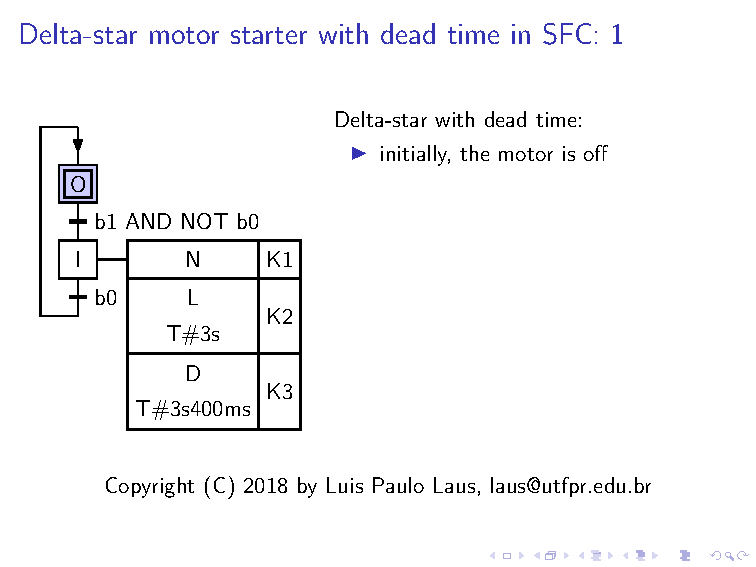
\includepdf[pages=-,offset=-116 285,noautoscale]{BeamerAnimation.pdf}

\end{document}